\chapter{Estado del arte}
\label{estadoArte}

En el presente capítulo se describirán los conceptos fundamentales relacionados con el proyecto, así como las diversas herramientas que se utilizarán mayoritariamente. El propósito de este capítulo es establecer un marco teórico sólido que permita abordar el análisis y el diseño del protocolo de comunicación \textit{in-band} de manera óptima antes de su desarrollo. Finalmente, se hará referencia a las contribuciones y la documentación generada con el fin de difundir los contenidos del proyecto a través de la plataforma \textit{GitHub}.


%%%%%%%%%%%%%%%%%%%%%%%%%%%%%%%%%%%%%%%%%%%%%%%%%%%%%%%%%%%%%%%%%%%%%%%%%%%%%%%%%%%%%%%%%%%%%%%%%%%%%
% 6G
%%%%%%%%%%%%%%%%%%%%%%%%%%%%%%%%%%%%%%%%%%%%%%%%%%%%%%%%%%%%%%%%%%
\section{Red de comunicación \glsentryshort{6g}}
\label{sec:6g}

%%%%%%%%%%%%%%%%%%%%%%%%%%%%%%%%%%%%%%%%%%%%%%%%%%%%%%%%%%%%%%%%%%%%%%%%%%%%%%%%%%%%%%%%%%%%%%%%%%%%%
% IoT
\section{Tecnología \glsentryshort{iot}}
\label{iot}

La premisa básica de la tecnología \gls{iot} \cite{iotreview} conectar cualquier dispositivo que tenga cierta capacidad de cómputo. Esto significa que los objetos que actualmente no están conectados a Internet, estarán conectados de manera que puedan comunicarse e interactuar con personas y otros objetos. \\
\par

La tecnología \gls{iot} es una transición tecnológica en la que los dispositivos al ser dotados de inteligencia por estar conectados a Internet podrán proveer de entornos inteligentes a los humanos.  Cuando los objetos puedan ser controlados a distancia a través de una red, se habilitará una integración más estrecha entre el mundo físico y las máquinas, permitiendo mejoras en las áreas de medicina, automatización y logística \cite{7073822}.\\
\par

El ecosistema \gls{iot} es amplio, e incluso se puede parecer un poco caótico debido a la gran cantidad de componentes y protocolos que abarca. Es recomendable en vez de ver el \gls{iot} como un termino único, verlo como un paraguas de varios conceptos, protocolos y tecnologías, enfocados a un mismo propósito de interconectar ``Cosas" a Internet. Si bien la amplia mayoría de elementos \gls{iot} están diseñados para aportar numerosos beneficios en las áreas de productividad y automatización, al mismo tiempo introducen nuevos desafíos, como por ejemplo la gestión de la gran cantidad de dispositivos que van a aparecer en las redes, y la cantidad de datos y mensajes que todos estos generaran \cite{iotreview}.

\subsection{Arquitectura}

Aunque en el ecosistema hay diferentes \textit{stacks} de protocolos, todos ellos se pueden resumir en la siguiente arquitectura básica \cite{iotreview}.

\begin{itemize}
    \item \textit{Perception Layer}, en esta capa se da un significado físico a cada objeto. Consiste en sensores de diferentes tipos como etiquetas RFID, sensores IR u otras redes de sensores que podrían detectar la temperatura, la humedad, la velocidad y la ubicación, etc. Esta capa recolecta información útil a partir de los sensores vinculados a los objetos,  convierte dicha información en señales digitales que más tarde se delegarán a la Capa de Red para su posterior transmisión.
    
    \item \textit{Network Layer}, el propósito de esta capa es la de recibir la información en
    forma de señales digitales desde la capa de Percepción y transmitirla a los sistemas de procesamiento en la capa de \textit{Middleware}. Esto se llevará a cabo a través de las distintas tecnologías de acceso como WiFi, BLE, WiMaX, ieee802154 y con protocolos como IPv4, IPv6, MQTT.
    
    \item \textit{Middlware Layer}, en esta capa se procesa la información recibida de todos los sensores. En esta capa se puede incluir las tecnologías como Cloud computing, o sistemas gestores,  que aseguran un acceso directo a bases de datos donde se puede almacenar toda la información recolectada. Teniendo una gran cantidad de información centralizada, generalmente se aplican sistemas de inteligencia artificial para procesar la información, y tomar decisiones predictivas totalmente automatizadas. Estos sistemas suelen ser utilizados para analizar el tiempo, contaminación o tráfico en las ciudades. 
    
    \item \textit{Application Layer}, la finalidad de  esta  capa es la de realizar las aplicaciones \gls{iot} para el usuario final. Estas aplicaciones se valdrán de los datos procesados para ofrecer funcionalidades al usuario final, por ejemplo, una aplicación del tiempo.
    
    \item \textit{Business Layer}, esta capa aunque es un poco abstracta, se suele añadir para representar la gestión de múltiples las aplicaciones y servicios \gls{iot}. 
\end{itemize}

% Foto 
\begin{figure}[ht]
    \centering
    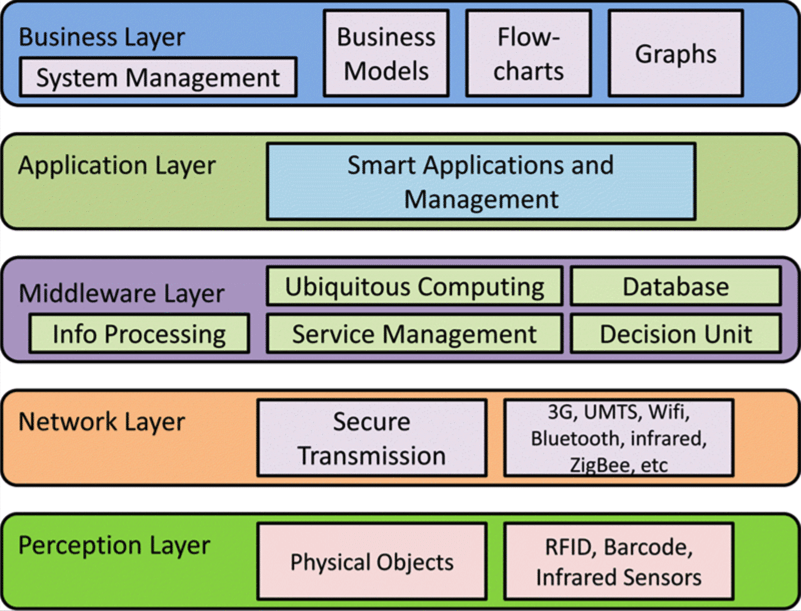
\includegraphics[width=6.5cm]{archivos/img/teoria/arch_edited.png}
    \caption{Arquitectura básica \glsentryshort{iot}}
    \label{fig:iotBasicArch}
\end{figure}

\subsection{Topologías}

Entre las tecnologías de acceso disponibles para conectar los dispositivos de \gls{iot}, dominan tres esquemas topológicos principales, estrella, malla y p2p. Para las tecnologías de acceso de largo y corto alcance, predomina la topología de estrella, como se puede encontrar en las redes datos móviles, LoRa y BLE. Las topologías en estrella utilizan una única estación base central para permitir las comunicaciones con los nodos finales. En cuanto a las tecnologías de mediano alcance, se pueden encontrar topologías en estrella, de p2p o en malla, como se ve en la figura \ref{fig:iotTopo}. Generalmente se suele hacer uso de un tipo de topología sobre otra en función de las limitaciones de los nodos que la conforman \cite{iotbook}.\\
\par

% Foto 
\begin{figure}[ht]
    \centering
    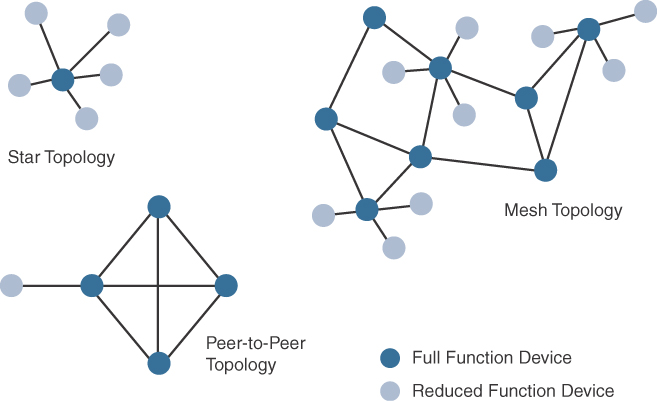
\includegraphics[width=7.5cm]{archivos/img/teoria/iot_topo.jpg}
    \caption{Tipos de topología con dispositivos \glsentryshort{iot} \cite{iotbook}}
    \label{fig:iotTopo}
\end{figure}


\subsection{Redes LLN}

Las redes de baja capacidad, conocidas como, \gls{lln}\footnote{\url{https://tools.ietf.org/html/rfc7228}}, se caracterizan por estar compuestas de dispositivos (sensores, motas) con limitaciones de memoria, batería y procesamiento. Dichos nodos, se interconectarán haciendo uso de distintos de tipos de enlace, como por ejemplo \texttt{ieee802154} ó LowPower-WiFi \cite{llnrfc}. Este tipo de redes pueden estar presentes en distintos campos de aplicación, entre las que se incluyen asistencia sanitaria, monitorización industrial, redes de sensores, etc.   \\

\par
Otra condición de las redes \gls{lln}, son las pérdidas en capa física debidas a las interferencias y variabilidad de los ``complicados" entornos radio donde estarán desplegadas dichas redes. Por ello, y teniendo en cuenta que los nodos que formarán parte de las redes \gls{lln} serán de baja capacidad, es necesario que los protocolos utilizados en esta red sean capaces de optimizar al máximo los recursos de los dispositivos \cite{iotbook}. 

\subsubsection{IEEE 802.15.4}

El estándar \texttt{ieee802154}\footnote{\url{https://tools.ietf.org/id/draft-ietf-lwig-terminology-05.html}} define la tecnología acceso a un entorno inalámbrico (\textit{phy} y \textit{mac}) para dispositivos de baja capacidad (limitados en batería y capacidad de transmisión). Este estándar se caracteriza por la optimización de los recursos del nodo en cuestión, consiguiendo una duración prolongada de la batería, además, esta tecnología de acceso permite un fácil uso utilizando un \textit{stack} de protocolos compacto, al tiempo que sigue siendo simple y flexible. Por todas estas características, el estándar \texttt{ieee802154} es usado en la mayoría de \textit{stack} de protocolos enfocados al \gls{iot}. Uno de los más utilizados es el \textit{stack} 6LoWPAN, definido por el \gls{ietf}, consiste en una capa de adaptación de IPv6 sobre las capas del estándar \texttt{ieee802154} (Ver figura \ref{fig:6lowapan}) \cite{6lowpan}.\\
\par

\vspace{0.5cm}

% Foto 
\begin{figure}[ht]
    \centering
    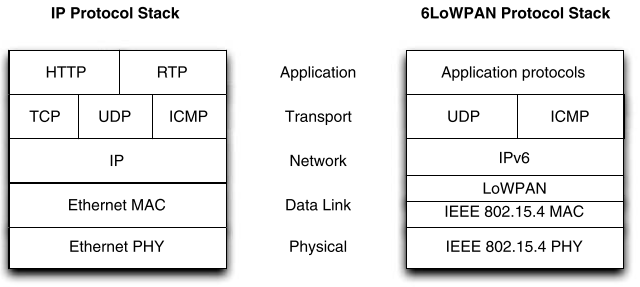
\includegraphics[width=12cm]{archivos/img/teoria/6LoWPAN-Protocol-Stack.png}
    \caption{Pila de protocolos 6LoWPAN \cite{6lowpan}}
    \label{fig:6lowapan}
\end{figure}



%%%%%%%%%%%%%%%%%%%%%%%%%%%%%%%%%%%%%%%%%%%%%%%%%%%%%%%%%%%%%%%%%%%%%%%%%%%%%%%%%%%%%%%%%%%%%%%%%%%%%
% SDN
\section{Redes  \glsentryshort{sdn}}
\label{sec:sdn}


El paradigma \gls{sdn} \cite{nadeau2013sdn} consiste en una arquitectura de red donde se lleva a cabo la separación del plano de control de la red para centralizarlo en un único ente llamado controlador. De esta forma se consigue que la administración de red sea una tarea más centralizada y flexible \cite{nadeau2013sdn}. La idea del \gls{sdn} empezó a germinar en la Universidad de Stanford por el año 2003, donde el profesor asociado en su momento, Nick McKeown, planteaba las limitaciones de las redes convencionales y veía la necesidad de replantear como los \textit{backbones} debían operar \cite{sdnBegins}. Dicha idea se acuñó como \gls{sdn} en el año 2011, cuando a la par se lanzó la organización \gls{onf} \cite{onf} como un portador de los estándares relacionados con el \gls{sdn} y su difusión.

\subsection{Arquitectura}

La arquitectura \gls{sdn} destaca por ser dinámica, rentable y adaptable haciéndola ideal para las demandas presentadas hoy en día por las redes de comunicaciones. Como ya se ha comentado, la arquitectura se basa en separar el plano de control del plano de datos, y llevar ese plano de control a una entidad llamada controlador. Desde dicha entidad se ofrecerán las interfaces necesarias para que aplicaciones de servicios de red puedan hacer uso de ellas. De esta forma, el control de la red se vuelve directamente programable, consiguiendo que la gestión se vuelva más ágil y dinámica.\\
\par

Como se puede ver en la figura \ref{fig:sdnBasicArch}, la arquitectura \gls{sdn} se divide en tres capas, la primera, el plano de datos que contendrá todos los elementos de red que habiliten el forwarding. La segunda, el plano de control, compuesto de los distintos controladores de la red \gls{sdn}, y por último, la capa de aplicación, en la cual se encontrarán todas las aplicaciones que se comuniquen con el controlador \gls{sdn}. \\
\par
Dichas capas se comunicarán entre ellas a través de interfaces abiertas. Por ejemplo, la interfaz \textit{Southbound} permite programar el estado de reenvío de los elementos de red del plano de datos. En cambio, la interfaz \textit{Northbound} comunica las aplicaciones con los controladores \gls{sdn}, habilitando la obtención de datos o el ajuste de parámetros a través de una API-Rest. También se pueden encontrar otro tipo de interfaces, \textit{Westbound} y \textit{Eastbound}, que se han consolidado los últimos años para la interconexión de controladores con la finalidad de establecer una misma política entre distintos dominios \gls{sdn}.

% Foto 
\begin{figure}[ht]
    \centering
    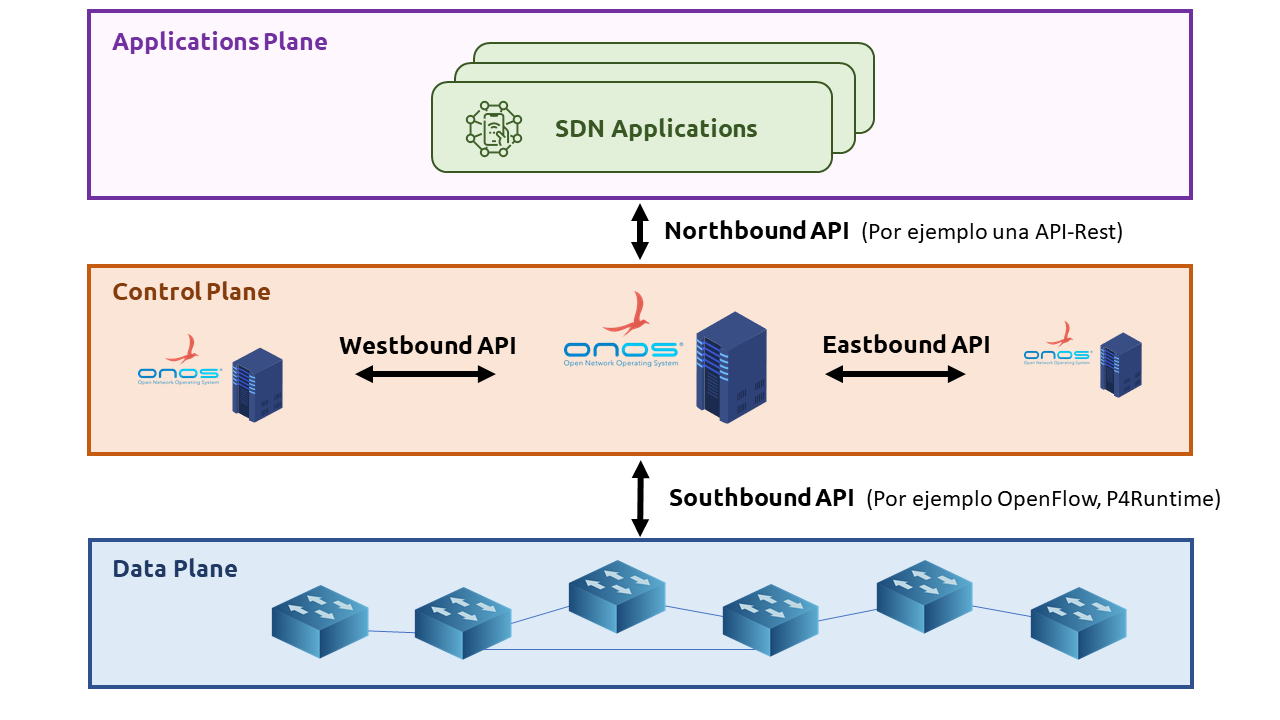
\includegraphics[width=14.5cm]{archivos/img/teoria/sdn_arch.png}
    \caption{Arquitectura básica \glsentryshort{sdn}}
    \label{fig:sdnBasicArch}
\end{figure}

\subsection{OpenFlow}

Existen varios protocolos para el control de los elementos de red desde el controlador, pero el más utilizado es Openflow. OpenFlow es un protocolo de la interfaz \textit{Southbound} que comunica los controladores \gls{sdn} con los elementos de red para configurar el estado de reenvío de estos últimos. La especificación de este protocolo se encuentra recogida por la \gls{onf}\footnote{\url{https://www.opennetworking.org/software-defined-standards/specifications/}}, contando con numerosas versiones siendo la última la versión \texttt{1.5.1} del 2015. \\
\par

El elemento clave de OpenFlow es el flujo (\textit{flow}), los cuales se conforman de paquetes que ha sido clasificados en función de reglas. Dichas reglas se encuentran en las tablas de flujo (\textit{flow table}) y  suelen estar relacionadas con los puertos de entrada o valores de cabecera típicos. Cuando estos criterios coinciden con los del paquete entrante se produce un \textbf{\textit{match}}.\\
\par
En el momento en que se produce un \textit{match}, el paquete en cuestión se verá sujeto a una serie de instrucciones asociadas a la regla con la que a hecho \textit{matching}. Estas instrucciones pueden ir desde, hacer una medición del paquete, aplicar una acción ó ir a otra tabla de flujo. De esta forma, con unas tablas de flujo completadas con unas reglas suministradas por el controlador \gls{sdn}, se conforma el estado de reenvío del switch en cuestión \cite{nadeau2013sdn}. 


%%%%%%%%%%%%%%%%%%%%%%%%%%%%%%%%%%%%%%%%%%%%%%%%%%%%%%%%%%%%%%%%%%%%%%%%%%%%%%%%%%%%%%%%%%%%%%%%%%%%%
% Controladores SDN (Ryu & Onos)
\section{Controladores \glsentryshort{sdn}}
\label{sec:sdnControllers}

Los controladores \gls{sdn}, también conocidos como sistemas operativos de red, son una pieza clave en los entornos  \gls{sdn} dado que tienen una vista global de toda la red que gestionan, que flujos atraviesan la red, estadísticas, usuarios finales, modelos y características de dichos equipos. Este controlador tiene la funcionalidad de interconectar los recursos disponibles en la red que gestiona, a aplicaciones o servicios que corran encima de él \cite{nadeau2013sdn}. De esta forma, cada vez que se quiera añadir una nueva funcionalidad, solo se tendrá que programar un nuevo servicio que corra encima del controlador que gestiona la red, y este a su vez se encargará de traducir las demandas del servicio a políticas de red a cada dispositivo impactado. En este matiz se puede llegar apreciar el sentido de nombre del paradigma \gls{sdn}, ya que estamos definiendo por software el comportamiento intrínseco de la red.\\
\\
% fig
\begin{figure}[ht]
    \centering
    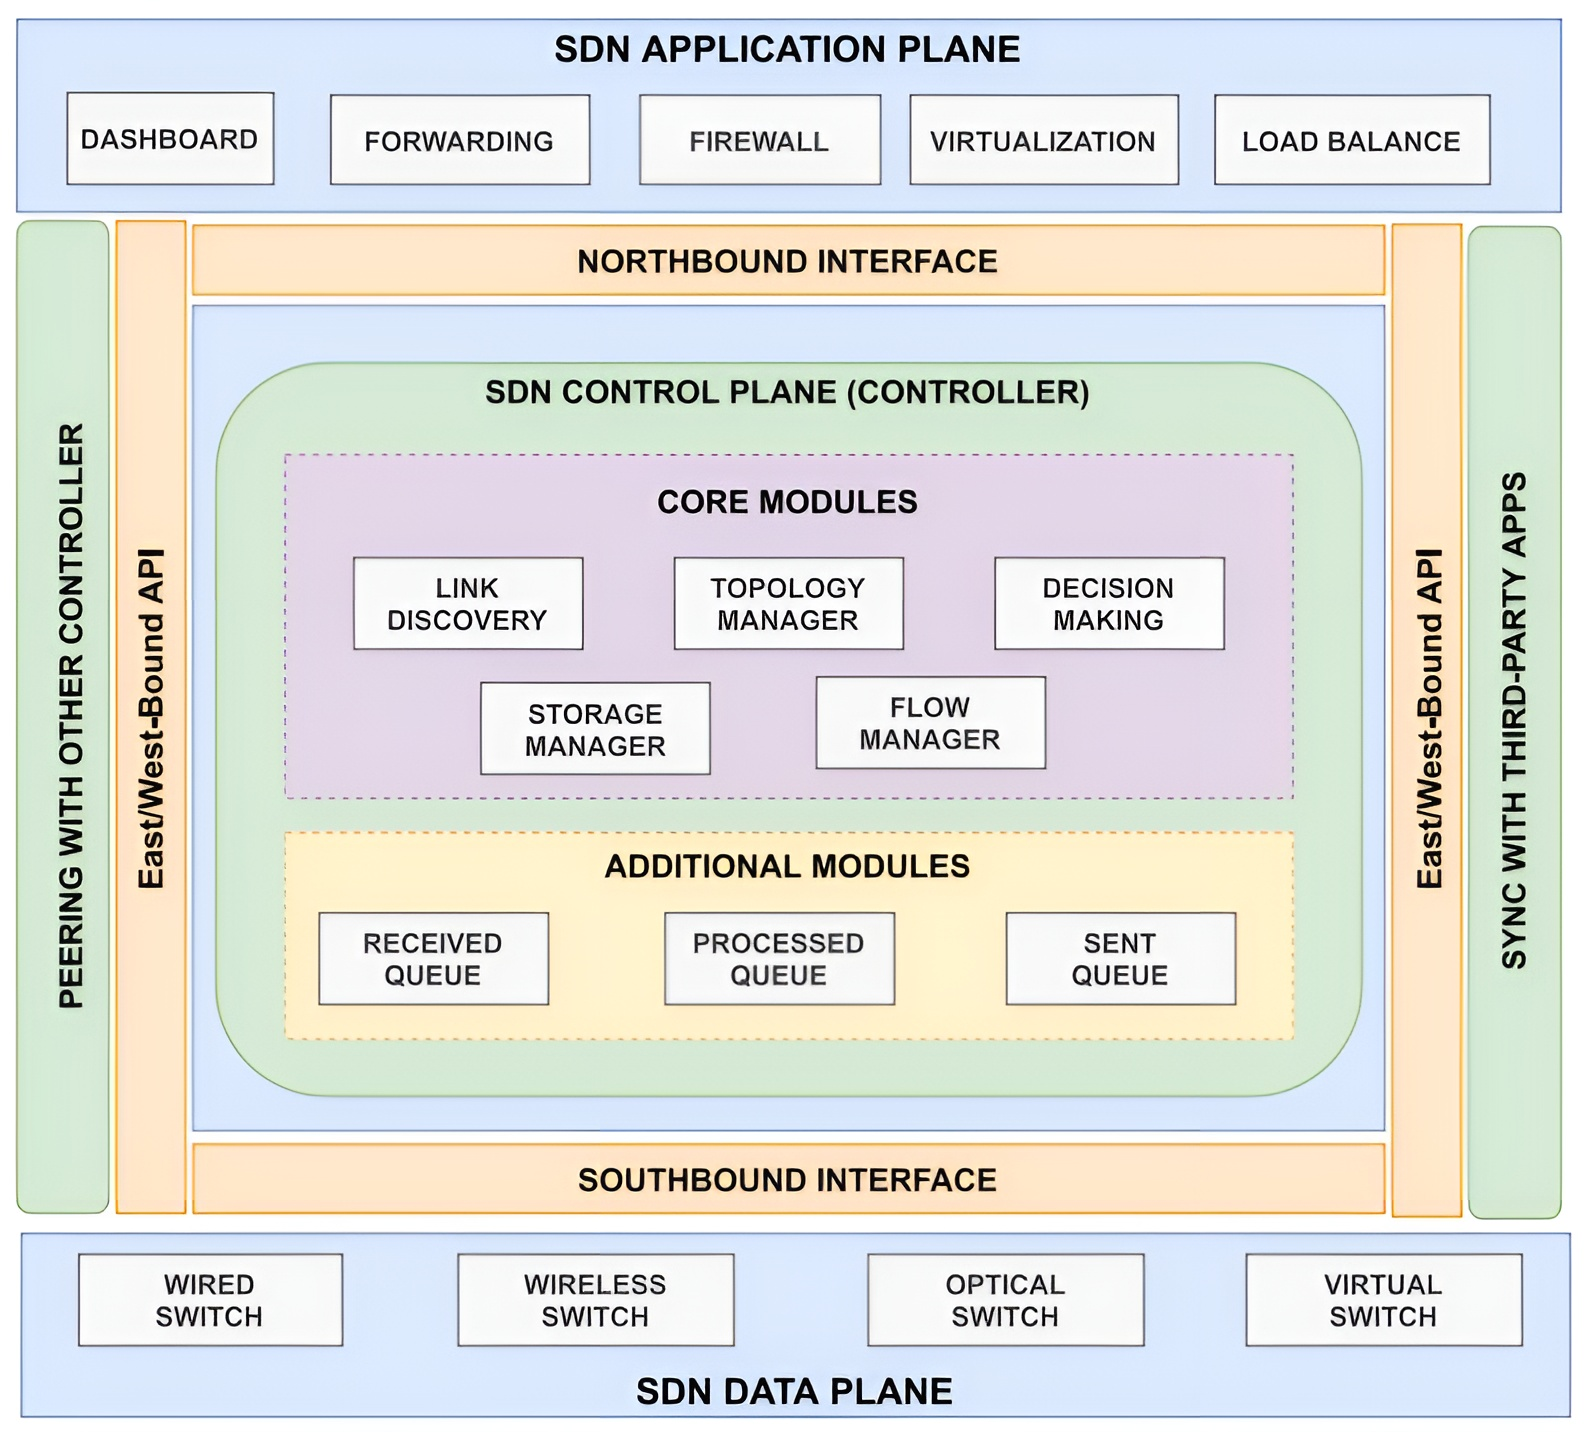
\includegraphics[width=\textwidth]{archivos/img/teoria/sdn_controllers.jpg}
    \caption{Arquitectura generica de controlador \glsentryshort{sdn} \cite{zhu2020sdn}}
    \label{fig:sdn_controllers}
\end{figure}

En la literatura hay muchas propuestas de arquitecturas para los controladores, pero en vez de ir una por una viendo las diferencias vamos a presentar la arquitectura genérica que se puede encontrar en la gran mayoría de controladores \gls{sdn}. Si nos fijamos en la Figura \ref{fig:sdn_controllers}, podemos ver dos partes claramente diferenciadas, el núcleo del controlador y las interfaces del mismo \cite{zhu2020sdn}. Empezando por el \textit{core}, se puede resumir que las funciones básicas del controlador están relacionadas principalmente con el descubrimiento de la topología y la gestión de los flujos de tráfico. El módulo de descubrimiento de la topología suele trabajar con el protocolo \gls{lldp}. La implementación puede variar entre controladores y aplicaciones de descubrimiento topológico, pero en términos generales, se transmite regularmente consultas utilizando mensajes \texttt{packet\_out}, los cuales viajaran por la topología física y volverán al controlador en forma de mensajes \texttt{packet\_in}, que permiten al controlador construir la topología de la red.\\
\\
Una vez que se conoce la topología de red, el controlador puede empezar a poner en marcha distintos módulos de toma de decisiones para encontrar los caminos óptimos entre los nodos de la red. Con todos los caminos ya construidos, entran en juego otros módulos del controlador como son \gls{qos} y de seguridad, los cuales pueden optar por instalar una ruta sub-óptima para satisfacer los criterios de \gls{qos} o de seguridad. De forma adicional, el controlador puede tener un recopilador de estadísticas y un gestor de colas para recopilar información sobre el rendimiento de las diferentes colas de paquetes entrantes y salientes de los dispositivos de red que gestiona, y con ellos realimentar a los módulos de \gls{qos}. Por último, tenemos uno de los módulos más importantes del controlador, el gestor de flujos. El gestor de flujos, puede variar su implementación en función de los protocolos que se utilicen en la \gls{sbi}, pero su misión es la misma, instalar reglas en los dispositivos de red que gestiona las directrices necesarias para gestionar los paquetes de un determinado flujo de una determinada manera. \\
\\
Siguiendo con otra parte fundamental del controlador \gls{sdn} genérico, son las interfaces. El controlador está rodeado de interfaces para interactuar con otras capas, superior e inferior, y otros controladores, este y oeste (E-WBIs). Empezando por la interfaz \gls{sbi}, la cual es la encargada de interconectar dispositivos \gls{sdn} con el controlador, define un conjunto de reglas, que variarán en función del protocolo que se utilice, las cuales permiten definir el procesamiento y las políticas de reenvío de los dispositivos \gls{sdn}. El protocolo OpenFlow es unas de las \gls{sbi} más utilizadas, y es un estándar de facto para la industria, con el cual podemos es definir flujos y clasificar el tráfico de red basándose en un conjunto de reglas predefinidas. Pero también se pueden encontrar otras \gls{sbi}, como por ejemplo, P4Runtime de facto el futuro para las \gls{sbi}s, o podemos encontrar algunas más \textit{legacy}, como por ejemplo, Netconf o incluso \gls{snmp}.\\
\\
Si nos vamos de la API sur, al norte, encontraremos la conocida como \gls{nbi}, la cual interconecta el controlador \gls{sdn} con las aplicaciones de los desarrolladores o los servicios que definan el comportamiento intrínseco de la red. Los controladores admiten varias interfaces de programación de aplicaciones (API) northbound, pero la mayoría de ellas se basan en la API REST. Generalmente se quiere que la interfaz \gls{nbi} sea una interfaz genérica para que limite a los desarrolladores. Para la comunicación entre controladores, se utilizan las interfaces conocidas como de este y oeste (E/WBI), las cuales no tienen una interfaz de comunicación estándar, por lo que, en función del controlador se tendrá una implementación u otra.\\
\\
A continuación, se presentan dos de los controladores \gls{sdn} más populares: Ryu y \gls{onos}, indicando algunas de sus virtudes y funcionamiento en particular, si bien existen otros como Floodlight, OpenDaylight, etc.

\subsection{Ryu}
\label{subsec:ryu}

Ryu\footnote{Del Japonés, significa ``flujo" y también ``dragón", ambos símbolos Kanji se leen igual como RYU, de ahí que el logo sea un dragón.} es un controlador de red de código abierto diseñado específicamente para redes \gls{sdn}. Se desarrolló en Python por el equipo de NTT (\textit{Nippon Telegraph and Telephone}) y proporciona una plataforma flexible, sencilla y extensible para desarrollar aplicaciones de red basadas en SDN. Como se comentó anteriormente, la funcionalidad primordial que lleva a cabo es la de ser un intermediario entre los elementos de red, como por ejemplo switches SDN o nodos virtuales, y las aplicaciones o servicios que controlan la red a través de la \gls{nbi} \cite{tomonori2013introduction}. De esta forma, a través de la \gls{nbi}, permite a los desarrolladores programar el comportamiento de la red de manera dinámica y centralizada, facilitando la implementación de políticas de red, la configuración de routing y la gestión de tráfico.\\
\\
Ryu es altamente modular y proporciona una API bien definida que permite a los desarrolladores construir aplicaciones de red personalizadas hasta el más mínimo nivel. También es compatible con varios protocolos de comunicación utilizados en SDN, como OpenFlow (versiones \texttt{1.0, 1.2, 1.3, 1.4, 1.5}), NETCONF y OF-config \cite{tomonori2013introduction}.  Las aplicaciones Ryu son entidades que implementan varias funcionalidades dentro de Ryu y se comunican entre sí a través de eventos. Los eventos sirven como mensajes intercambiados entre las aplicaciones Ryu. Estas aplicaciones se envían eventos asíncronos entre sí, creando un flujo de comunicación. Además de las aplicaciones Ryu, existen ciertas fuentes de eventos internas al propio Ryu. Un ejemplo de estas fuentes de eventos es el controlador OpenFlow. Cada aplicación Ryu posee una cola de recepción específicamente diseñada para eventos. La cola funciona según el principio \gls{fifo}, lo que garantiza que se mantenga el orden de los eventos. Para procesar estos eventos, cada aplicación Ryu tiene un único hilo dedicado responsable de la gestión de eventos. Este subproceso vacía continuamente la cola de recepción retirando los eventos de la cola e invocando al manejador de eventos apropiado en función del tipo de evento \cite{ryu1}.

% fig
\begin{figure}[ht]
    \centering
    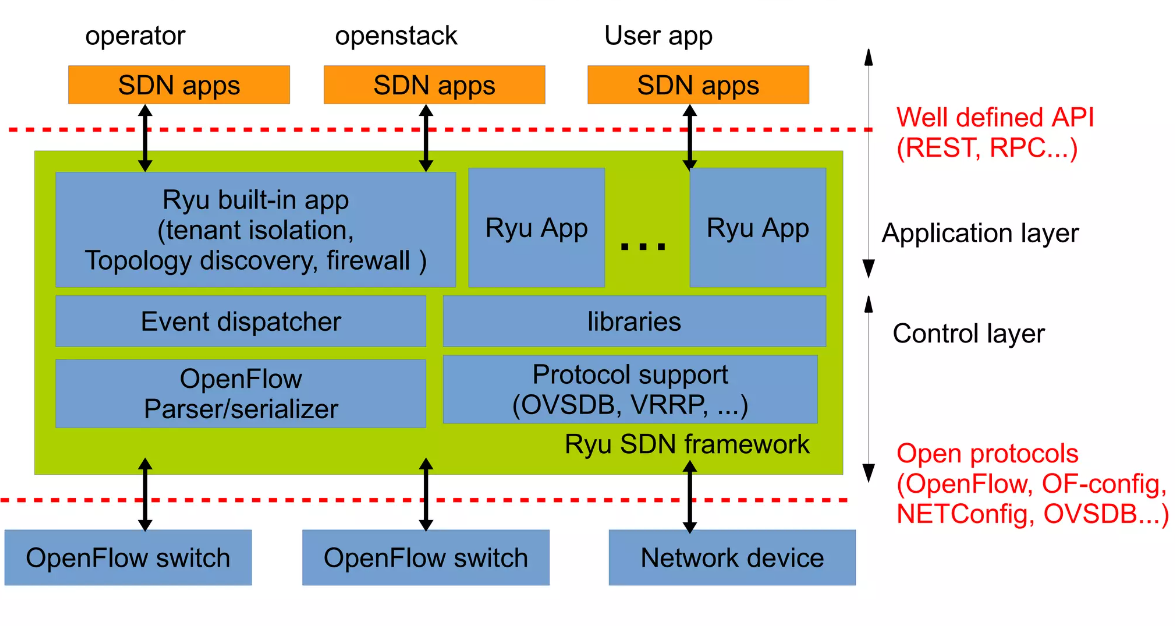
\includegraphics[width=0.85\textwidth]{archivos/img/teoria/ryu.png}
    \caption{Arquitectura del controlador \glsentryshort{sdn} RYU \cite{ryu2}}
    \label{fig:ryu}
\end{figure}

En la Figura \ref*{fig:ryu}, se puede apreciar como la arquitectura del controlador está divida en dos grandes bloques de acuerdo se han estudiado los controladores \gls{sdn}, la parte de \textit{core} y la parte de interfaces. En la parte del núcleo se puede apreciar como se a programado todas las librerías y el manejador de eventos que se mencionaba anteriormente. Por otro lado también se puede apreciar las capas de adaptación a la \gls{sbi} y a la \gls{nbi}, la primera de ellas se adapta a través de una API REST a servicios de aplicaciones externas, mientas que la interfaz \gls{sbi} implementa todos los protocolos de control \gls{sdn}. Algunas de las características y funcionalidades de Ryu incluyen:

\begin{itemize}
    \item Compatibilidad con múltiples protocolos SDN de la interfaz \gls{sbi}.
    \item Capacidad para implementar políticas de red y reglas de enrutamiento de forma sencilla.
    \item Soporte para la recopilación y el análisis de datos de red en tiempo real.
    \item Funcionalidad de control de \gls{qos}.
    \item La más importante de todas, fácil desarrollo y portabilidad sencilla al estar escrita en Python. Esta última se puede ver también como una desventaja, dado el pobre rendimiento de un lenguaje interpretado.
\end{itemize}

Ryu es utilizado en una amplia gama de entornos, desde laboratorios de investigación hasta en las clases de forma educativa. Esta herramienta suele ser el punto de estrada para muchas personas que se inician en el \gls{sdn}, sin embargo, al tener un pobre rendimiento, y la falta de abstracción con los protocolos que se usen en la interfaz \textit{southbound}, hace que en entornos comerciales no se suela ver con tanta frecuencia \cite{tomonori2013introduction}.

\subsection{ONOS}
\label{subsec:ONOS}

\gls{onos} es un controlador de red de código abierto diseñado específicamente para redes \gls{sdn}. Como su nombre indica, \gls{onos} es un sistema operativo para redes que proporciona funcionalidades avanzadas de control y gestión de redes. \gls{onos} está diseñado para ser escalable, confiable y de alto rendimiento, lo que lo hace adecuado para despliegues de red a gran escala. Es compatible con una amplia variedad de protocolos y tecnologías de red, como OpenFlow, NETCONF, BGP y \gls{p4} \cite{onos3}. El controlador está respaldado por la \gls{onf}, la cual es una organización sin ánimo de lucro fundada en 2011 con el objetivo de promover y acelerar la adopción de la tecnología \gls{sdn} y el enfoque de redes abiertas. Además de la \gls{onf}, numerosos proveedores de internet están impulsando el proyecto, así como, grandes empresas del sector TIC. Se pueden resumir las principales características y funcionalidades de \gls{onos} en los siguientes puntos.

\begin{itemize}
    \item  Control centralizado de la red: \gls{onos} proporciona un punto central lógico de control  para la gestión de toda la red. Permite la configuración dinámica de la red, el enrutamiento y la asignación de recursos.
    \item Escalabilidad: \gls{onos} está diseñado para manejar redes de gran escala, distribuyendo la carga de trabajo entre múltiples nodos para lograr un rendimiento óptimo y una alta disponibilidad.
    \item Programabilidad: \gls{onos} permite a los desarrolladores crear aplicaciones personalizadas utilizando una amplia gama de APIs y marcos de desarrollo. Esto facilita la implementación de políticas de red, la orquestación de servicios y la integración con otras aplicaciones y sistemas.
    \item Gestión de topología: \gls{onos} proporciona una visión global de la topología de la red, permitiendo el descubrimiento de dispositivos, enlaces y rutas. Esto facilita la toma de decisiones basadas en el estado actual de la red.
    \item Gestión de flujos: \gls{onos} admite la programación y gestión de flujos de red, lo que permite la implementación de políticas de enrutamiento y \gls{qos} de manera dinámica y centralizada.
    \item Segmentación de red: \gls{onos} es compatible con la segmentación de red, lo que permite crear \textit{network slices} para proporcionar aislamiento y asignación de recursos personalizada en una infraestructura compartida.
\end{itemize}

\gls{onos} se concibe como un sistema operativo de red completo que va más allá de ser solo un controlador \gls{sdn}. Ofrece una amplia gama de funcionalidades que incluyen herramientas como APIs que proporcionan abstracción para el desarrollo de aplicaciones \gls{sdn}, así como APIs para la administración, supervisión y programación de dispositivos de red. Además, \gls{onos} ofrece capacidades de virtualización, aislamiento, acceso seguro y abstracción de los recursos de red administrados por el sistema operativo. \gls{onos} tiene la capacidad de multiplexar recursos tanto hardware como software entre las aplicaciones \gls{sdn}, permitiendo una utilización eficiente de los recursos disponibles. Además, facilita la configuración de políticas de red basadas en las intenciones de las aplicaciones, lo que implica la aplicación de políticas de red diseñadas para satisfacer los requisitos específicos de las aplicaciones, así como el procesamiento de eventos de red \cite{onos2}. \\
\\
Si nos fijamos en la Figura \ref*{fig:onos}, podemos ver que este sistema operativo está diseñado para operar con dispositivos de red \textit{whitebox}, con el objetivo de reducir los costes asociados con las soluciones propietarias. \gls{onos} posee una arquitectura flexible que facilita la integración sencilla de nuevos dispositivos de hardware en el framework \gls{sdn}. Solo se requiere que se añada un driver del equipo o target propietario.  Además, puede funcionar como un sistema distribuido a través de múltiples servidores en modo cluster, lo que permite aprovechar los recursos de CPU y memoria de varios equipos simultáneamente. Esta capacidad también proporciona resiliencia ante posibles fallos de los servidores y permite realizar cambios en hardware y software sin interrumpir el tráfico de red \cite{onos1}.

% fig
\begin{figure}[ht]
    \centering
    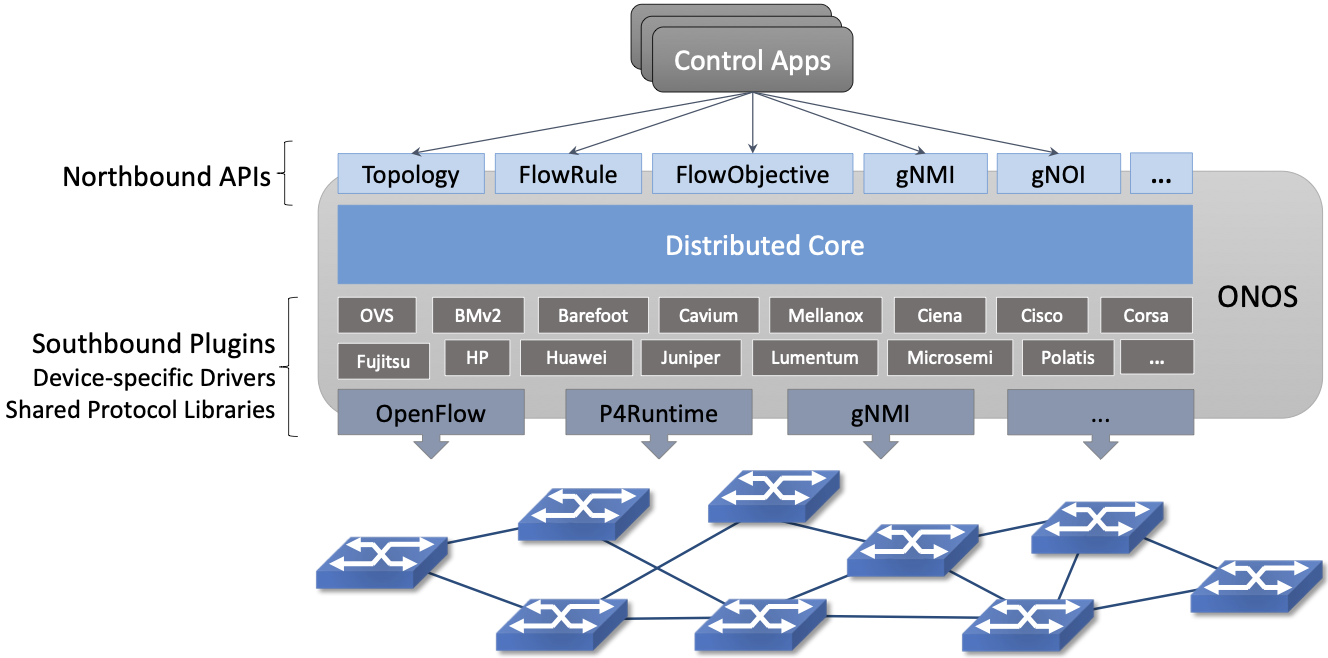
\includegraphics[width=\textwidth]{archivos/img/teoria/onos.png}
    \caption{Arquitectura del controlador \glsentryshort{sdn} onos \cite{onos1}}
    \label{fig:onos}
\end{figure}

\gls{onos} cuenta con una comunidad activa de desarrolladores y usuarios que contribuyen al desarrollo y mejora del sistema. Además, \gls{onos} es utilizado en diversos casos de uso, como redes de transporte, redes de centros de datos y redes de telecomunicaciones, entre otros muchos casos de uso. Si bien es cierto que tiene un muy buen rendimiento, no es controlador sencillo de manejar, y la curva de aprendizaje puede ser bastante pronunciada.

%%%%%%%%%%%%%%%%%%%%%%%%%%%%%%%%%%%%%%%%%%%%%%%%%%%%%%%%%%%%%%%%%%%%%%%%%%%%%%%%%%%%%%%%%%%%%%%%%%%%%
% Switches OVS & BOFUSS
\section{Software Switches \glsentryshort{sdn}}
\label{sec:softSwitchs}

En las redes definidas por software, los software switches desempeñan un papel fundamental al permitir la virtualización y la gestión centralizada de las redes. Estos switches, a diferencia de los switches de hardware tradicionales, se implementan como software y se ejecutan en servidores convencionales. Un software switch en \gls{sdn}, en adelante \textit{softswitch}, es una entidad lógica que reside generalmente en una instancia virtual o en un servidor, y se comunica con el controlador \gls{sdn} para recibir instrucciones sobre cómo procesar los paquetes de datos que fluyen a través de la red. Al estar basados en software, estos switches pueden ser escalados y desplegados de manera flexible según las necesidades y demandas de la red. La principal ventaja de los \textit{softswitches} radica en su capacidad para adaptarse y responder de manera dinámica a las necesidades de la red. Pueden implementar diferentes funciones de red, como enrutamiento, conmutación, balanceo de carga y seguridad, a través de la instalación de reglas desde el controlador \gls{sdn}. \\
\\
% fig
\begin{figure}[ht]
    \centering
    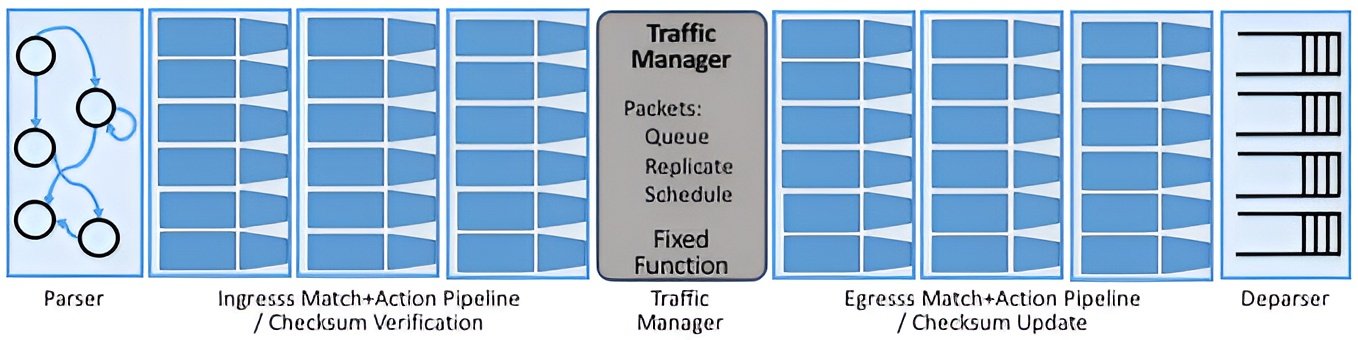
\includegraphics[width=0.8\textwidth]{archivos/img/teoria/softswitch.jpg}
    \caption{Arquitectura genérica de un \textit{softswitch} \gls{sdn} \cite{softswitches1}}
    \label{fig:softswitch}
\end{figure}

Según se puede apreciar en la figura \ref*{fig:softswitch}, la arquitectura genérica de un \textit{softswitch} se puede resumir en los siguientes bloques. El primero de todos tiene que ser un parser, que vaya inspeccionando los paquetes entrantes a la pipeline de procesamiento del switch para identificar que tipo es. Una vez se ha identificado el paquete que se va a procesar, el siguiente bloque son las tablas de \textit{match-action}, las cuales tienen una interfaz de comunicación con el controlador \gls{sdn} para establecer criterios y campos de \textit{match}, y en caso de haber un \textit{match}, definir una serie de acciones para llevar a cabo. En función del \textit{softswitch}, la verificación de \textit{checksum}\footnote{Suma de comprobación, campo para comprobar la integridad del paquete de datos} se puede llevar a cabo en el parser o en la etapa de las tablas de \textit{match-action}. El siguiente bloque que nos podemos encontrar en un \textit{softswitch} es el conocido como gestor de tráfico, que variará en función de la implementación, pero nos proveerá de gestión de colas, \gls{qos}, duplicado de paquetes, etc. La siguiente etapa ya es más opcional, que se suele denominar como \textit{egress match-action}, la cual se puede utilizar para definir algún tipo de lógica a la salida de los switches, aunque en la realidad se suele utilizar para actualizar los campos  de \texttt{TTL} y recalcular el \textit{checksum} dado que el paquete se habrá visto modificado. El último bloque es el deparser, el cual se encarga de ensamblar de nuevo el paquete y prepararlo para sacarlo por el puerto de salida del switch.

\subsection{OVS}
\label{subsec:OVS}

OVS (Open vSwitch) es un software switch de código abierto diseñado específicamente para su uso en redes definidas por software (SDN). Es uno de los software switches más utilizados y ampliamente adoptados en entornos SDN debido a su flexibilidad y funcionalidades avanzadas.

Open vSwitch actúa como un switch virtual, proporcionando capacidades de conmutación y enrutamiento para máquinas virtuales y contenedores en entornos de virtualización. Puede ejecutarse en hipervisores populares, como KVM (Kernel-based Virtual Machine), Xen y VMware, y también puede ser implementado como un switch independiente en sistemas operativos de servidor.

Las características clave de Open vSwitch incluyen:

1. Controlador SDN: Open vSwitch se puede controlar y programar mediante un controlador SDN, como OpenDaylight o ONOS. Esto permite una gestión centralizada y un control más granular de la red, así como la implementación de políticas de red definidas por software.

2. Funcionalidades avanzadas: OVS ofrece una amplia gama de funcionalidades, como enrutamiento, balanceo de carga, aislamiento de red, seguridad y calidad de servicio (QoS). Estas características permiten una gestión eficiente de la red y la implementación de políticas específicas para satisfacer las necesidades de las aplicaciones y usuarios.

3. Segmentación de red: Open vSwitch es compatible con la segmentación de red, lo que permite la creación de redes virtuales (network slices) dentro de una infraestructura compartida. Esto permite el aislamiento y la asignación de recursos personalizados para diferentes aplicaciones o usuarios, mejorando la seguridad y el rendimiento de la red.

4. Integración con tecnologías de virtualización: OVS se integra estrechamente con tecnologías de virtualización como OpenStack y Docker. Puede proporcionar conectividad de red entre máquinas virtuales, contenedores y hosts físicos, facilitando la migración y la gestión de recursos en entornos virtualizados.

5. Extensibilidad y soporte para estándares: Open vSwitch es altamente extensible y se puede ampliar mediante la integración de módulos y complementos personalizados. Además, cumple con los estándares de la industria, como el protocolo OpenFlow, para garantizar la interoperabilidad con otros componentes SDN.

En resumen, Open vSwitch (OVS) es un software switch SDN ampliamente utilizado que proporciona capacidades avanzadas de conmutación y enrutamiento para entornos de virtualización. Su flexibilidad, funcionalidades avanzadas, segmentación de red y compatibilidad con estándares lo convierten en una opción popular para implementaciones SDN en diversos entornos, desde centros de datos hasta infraestructuras de proveedores de servicios.

\subsection{BOFUSS}
\label{subsec:BOFUSS}

%%%%%%%%%%%%%%%%%%%%%%%%%%%%%%%%%%%%%%%%%%%%%%%%%%%%%%%%%%%%%%%%%%%%%%%%%%%%%%%%%%%%%%%%%%%%%%%%%%%%%
% Linux Networking
\section{Linux Networking}
\label{sec:linuxNetworking}

Esta sección recopilará todos los conceptos y herramientas relacionadas con la parte de Networking en Linux, que son fundamentales para el desarrollo, análisis y validación de este proyecto.


%%%%%%%%%%%%%%%%%%%%%%%%%%%%%%%%%%%%%%%%%%%%%%%%%%%%%%%%%%%%%%%%%%%%%%%%%%%%%%%%%%%%%%%%%%

\subsection{Interfaz virtual - \texttt{tun/tap}}
\label{linuxNetworking_tuntap}

En el mundo de las redes siempre se habla de las interfaces tun/tap de forma indistinta cuando van a utilizarse, sin embargo, cada una tiene su cometido. Como se ha indicado, en networking, las interfaces TUN y TAP son interfaces virtuales que se crean y se gestionan en espacio de kernel. Mencionar que como estas interfaces son virtuales y se gestionan directamente vía softaware, no como las interfaces reales que se gestionan con unos drivers diferentes, cada interfaz con su driver específico de la interfaz.  Los drivers de las interfaces TUN/TAP se crearon en los 2000 como una unión de los avances de los drivers desarrollados en las comunidades de Solaris, Linux, BSD. Actualmente los drivers solo tienen mantenimiento por los kernels de linux y FreeBSD. Ambos tipos de interfaces se utilizan para tunelado, pero no pueden ser utilizadas a la vez dado que trabajan en niveles distintos. Las TUN, de \textit{network \textbf{TUN}nel}, emula la capa de red y puede llegar hacer reenvío de los paquetes. En cambio las interfaces TAP,  trabajan en capa 2 solo en capa dos, y emulan un equipo que trabaja en dicha capa, como por ejemplo un switch. Por tanto, hay que dejar claro lo que se puede llegar a realizar con cada interfaz (Ver figura \ref{fig:linux1}).

\begin{itemize}
    \item \texttt{TUN} se puede llegar a utilizar para routing.
    \item \texttt{TAP} se puede llegara utilizar para crear un bridge.
\end{itemize}

Generalmente, cuando los paquetes son enviados por el sistema operativo a través de una interfaz TUN/TAP,  serán recibidos por algún programa de espacio de usuario, el cual, está enganchado directamente en la interfaz. Cualquier programa de espacio de usuario podrá pasar paquetes por las interfaces, y las interfaces virtuales se lo pasarán al \textit{stack} de red por defecto, emulando la recepción de los paquetes inyectados desde espacio de usuario.

% fig
\begin{figure}[ht]
    \centering
    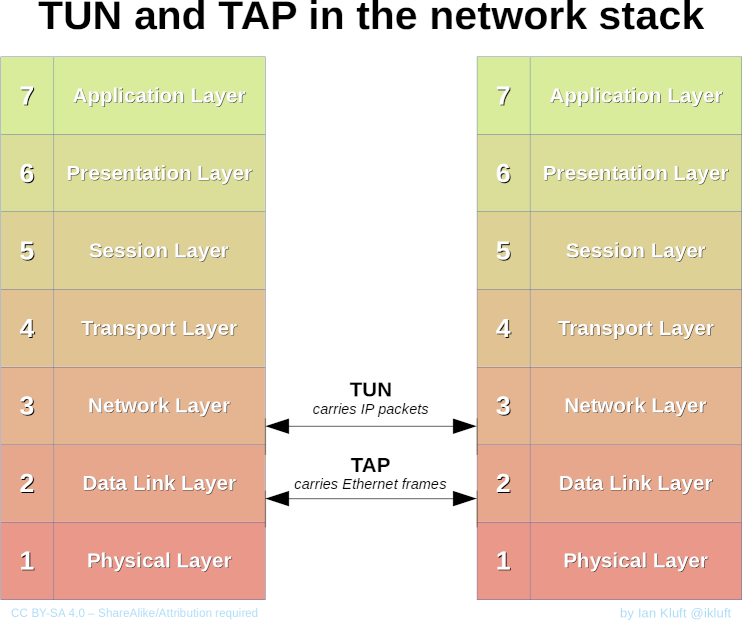
\includegraphics[width=\textwidth]{archivos/img/teoria/linux1.png}
    \caption{Diagrama de funcionamiento de las interfaces virtuales TUN/TAP }
    \label{fig:linux1}
\end{figure}

Para la creación de estas interfaces lo podemos hacer por ioctl o podemos hacerlo más fácil a través del binario tunctl o en su defecto con el comando de \texttt{tuntap} del set de herramientas iproute2. A continuación, en el bloque \ref{code:tun_tap_use} se indican todos los comandos necesarios para trabajar con las interfaces TUN/TAP.

\begin{lstlisting}[language= bash, style=Consola, caption={Manejo de interfaces TUN - TAP},label=code:tun_tap_use]
    # En caso de querer utilizar tunctl hay que instalar el binario
    sudo apt install -y uml-utilities
    
    # Para crear una un interfaz podemos hacer lo siguiente
    tunctl -t {nombre_tun}

    # Para eliminarla
    tunctl -d {nombre_tun}

    # Para crear interfaces de tipo TAP hay que hacer lo siguiente
    tunctl -p -t {nombre_tun}
    
    # El comando análogo con iproute2 sería el siguiente
    ip tuntap add dev {nombre_tun} mode {tun|tap}
\end{lstlisting}
\vspace{0.5cm}

En caso de que queramos comprobar que las interfaces se han creado correctamente siempre se puede hacer uso de la herramienta \texttt{ethtool}. A continuación, en la figura \ref{fig:linux2}, se puede ver como en el campo \texttt{bus-info} nos indica que tipo de interfaz es.

% fig
\begin{figure}[ht]
    \centering
    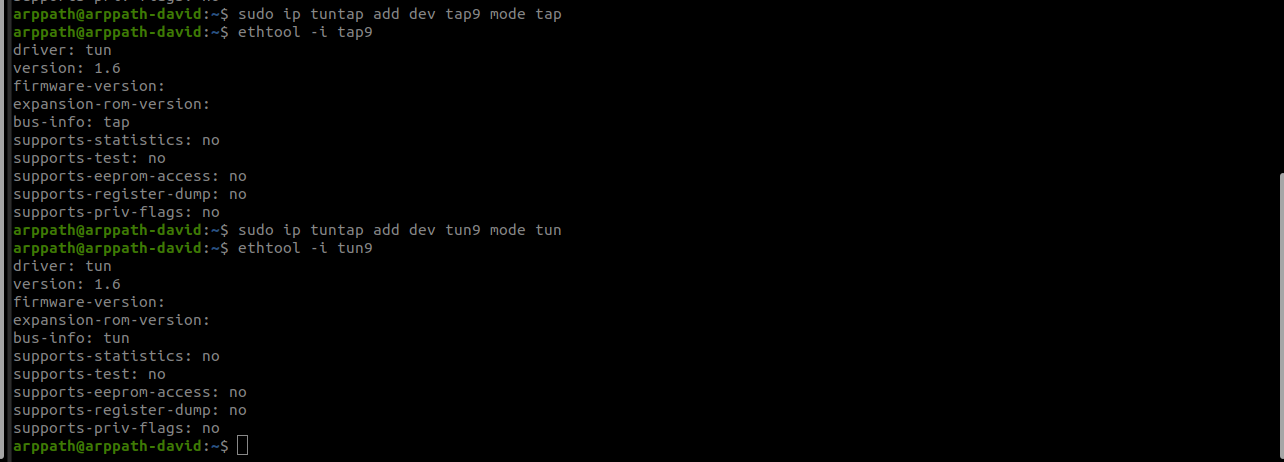
\includegraphics[width=\textwidth]{archivos/img/teoria/linux2.png}
    \caption{Comprobación con \texttt{ethtool} de tipo de interfaz virtual.}
    \label{fig:linux2}
\end{figure}


%%%%%%%%%%%%%%%%%%%%%%%%%%%%%%%%%%%%%%%%%%%%%%%%%%%%%%%%%%%%%%%%%%%%%%%%%%%%%%%%%%%%%%%%%%
\subsection{Interfaz virtual - \texttt{veth}}
\label{linuxVeths}
Las \gls{veth}, son interfaces de Ethernet virtuales creadas como un par de interfaces interconectadas entre si. El modelo funcional es sencillo, los paquetes enviados desde una son recibidos por la otra interfaz de forma directa, bastante parecido al funcionamiento de las \textit{pipes}. Una condición interesante de estas interfaces es que su gestión está asociada, es decir, si se levanta una extremo de la \gls{veth}, la otra también lo hará, si por el contrario se deshabilita o se destruye algún extremo de un par de \gls{veth} el otro extremo también se verá afectado \cite{veth}.\\
\par
Es muy común hacer uso de las \gls{veth} para interconectar \textit{Network Namespaces}, ya que, sabiendo que estas van a estar conectadas de forma directa, se puede utilizar este enlace como pasarela entre dos \textit{Network Namespaces}. De esta forma, se estaría interconectando dos \textit{stacks} independientes de red. La creación y destrucción de este tipo de interfaces se puede apreciar en el bloque \ref{code:iproute2_veth_use}, se recuerda que es necesario permisos de súper usuario.\\

\begin{lstlisting}[language= bash, style=Consola, caption={Manejo de Veths},label=code:iproute2_veth_use]
    # Crear un par veth
    ip link add {nombre_veth1} type veth peer name {nombre_veth2}
    
    # Si se elimina un extremo, el otro también lo hará
    ip link delete {nombre_veth}
    
\end{lstlisting}
\vspace{0.5cm}


%%%%%%%%%%%%%%%%%%%%%%%%%%%%%%%%%%%%%%%%%%%%%%%%%%%%%%%%%%%%%%%%%%%%%%%%%%%%%%%%%%%%%%%%%%

\subsection{Herramienta \texttt{TC}}


\gls{tc}, es un programa de espacio de usuario el cual es la pieza fundamental de la \gls{qos} en el Kernel de Linux. Muchas de sus funcionalidades se pueden resumir en cuatro puntos:

\begin{itemize}
    \item \textsc{SHAPING}
    \item \textsc{SCHEDULING}
    \item \textsc{POLICING}
    \item \textsc{DROPPING}
\end{itemize}

Según su \textit{man-page}\footnote{\url{https://man7.org/linux/man-pages/man8/tc.8.html}}, el procesamiento del trafico para conseguir dichas funcionalidades, se lleva a cabo con tres tipos de objetos: \textbf{qdiscs}, \textbf{classes} y \textbf{filters}.

\subsubsection{Qdiscs}

El objeto \gls{qdics}, disciplina de cola, es un concepto básico en el Networking de Linux que indica el orden en que los miembros de la cola, en este caso paquetes, se seleccionan para el servicio. Por ejemplo, en un momento dado puede que una herramienta de espacio de usuario requiera de transmitir un paquete, dicho paquete será entregado al \textit{stack} de red, llegando en última instancia a la interfaz de red por la cual va a ser transmitido. En ese momento el paquete se encontrará encolado en una cola de a la espera de ser trasnmitido, estas colas estarán regidas por un \gls{qdics}. El \gls{qdics} por defecto es un pfifo, es un puro \textit{first-in}, \textit{first-out} con limitación en el tamaño de cola en número de paquetes.


\subsubsection{Classes}

La clases se podrían ver como una sub-\gls{qdics} de una \gls{qdics}. Una clase puede contener a su vez otra clase, o más clases, pudiendo conformar sistemas de \gls{qos} en detalle, véase la figura \ref{fig:linuxNet_tc}. Cuando los paquetes son recibidos en una cola administrada por un \gls{qdics}, estos pueden ser encolados en base a las características del paquete en otras colas,  gestionadas por otras clases. Esto permite por ejemplo, priorizar el envío de datos de una aplicación sobre otra. Para ello, los paquetes de ambas aplicaciones se clasificarán en distintas clases, dándole más prioridad a una clase sobre la otra, asignándole más recursos de transmisión y recepción.

%foto
\begin{figure}[ht]
    \centering
    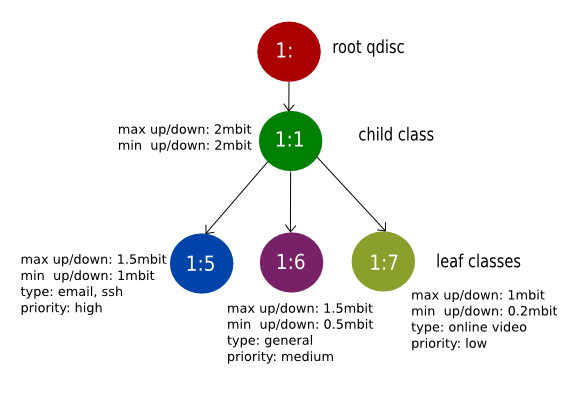
\includegraphics[width=8cm]{archivos/img/teoria/tc_qdisc_example_implementation.png}
    \caption{Sistema de QoS implementado con distintas clases \cite{qdiscs}}
    \label{fig:linuxNet_tc}
\end{figure}

\subsubsection{Filters}

Un filtro es usado para determinar con qué clase debe ser encolado el paquete. Para ello, el paquete siempre debe ser clasificado con una clase determinada. Varios tipos de filtros se pueden utilizar para clasificar los paquetes, pero en este caso será de interés el tipo de filtro \gls{bpf}\footnote{\url{https://man7.org/linux/man-pages/man8/tc-bpf.8.html}}, los cuales permiten anclar un \textit{bytecode} \gls{bpf}. Estos filtros se utilizarán para cargar programas \gls{bpf} que trabajarán en conjunto con \gls{xdp} con la finalidad de lograr el Broadcast. Esto es así, ya que en el \gls{tc} ya se hace uso de la estructura \texttt{sk\_buff} (Ir a \ref{linuxNetworking_skbuff}), por lo que ciertos \textit{helpers} \gls{bpf} para clonar paquetes podrán ser utilizados por \textit{bytecode} anclado en el filtro.


%%%%%%%%%%%%%%%%%%%%%%%%%%%%%%%%%%%%%%%%%%%%%%%%%%%%%%%%%%%%%%%%%%%%%%%%%%%%%%%%%%%%%%%%%%

\subsection{Namespaces}
\label{namespaces}
Una \textit{Namespace} se utiliza para aislar un recurso del sistema en una abstracción que hace  creer a los procesos dentro de dicha \textit{Namespace} que tienen su propia instancia del recurso en cuestión aislada del sistema real.  Los cambios realizados sobre recursos aislados del sistema, son solo visibles para procesos que son pertenecientes a la \textit{Namespace}, pero son invisibles para otros procesos pertenecientes al sistema o a otra \textit{Namespace}.\\
\par
Hay muchos tipos de \textit{Namespaces}, en la tabla \ref{tab:linux_ns} se pueden apreciar todos los tipos que existen a día de hoy. El uso de todos estos tipos de \textit{Namespaces} puede ser muy variado, pero el más importante de todos ellos son los contenedores. Los contenedores son elementos para correr aplicaciones, o herraminetas en un entorno aislado del sistema. A día de hoy, los contenedores más utilizados son los de Docker\footnote{\url{https://www.docker.com/}}, pero, ¿Realmente que hace Docker, qué es Docker?\\
\par

Docker se vale de las bondades del Kernel de Linux para aislar recursos y con esto conformar contenedores. Éste hará uso de las APIs suministradas por el Kernel para crear y destruir a conveniencia las distintas \textit{Namespaces}. Por lo que, Docker en verdad simplemente es un envoltorio de las llamadas al sistema para gestionar \textit{Namespaces}. Docker además, provee de distintos aspectos al usuario como \textit{copy-on-write}, o una configuración en modo \textit{bridge} hacia el exterior, pero en el fondo es
un mero \textit{wrapper} para la gestión de las \textit{Namespaces} con la finalidad de implementar contenedores.

% \begin{table}[ht]
%     \centering
%     \resizebox{\textwidth}{!}{%
%         \begin{tabular}{|l|l|}
%             \hline
%             \rowcolor[HTML]{EFEFEF}
%             \multicolumn{1}{|c|}{\cellcolor[HTML]{EFEFEF}{\color[HTML]{24292E} \textbf{Tipo de Namespace}}} & \multicolumn{1}{c|}{\cellcolor[HTML]{EFEFEF}{\color[HTML]{24292E} \textbf{Descripción}}}                                                                                                                                                     \\ \hline
%             \textbf{Cgroup}                                                                                 & \begin{tabular}[c]{@{}l@{}}Namespace utilizada generalmente para establecer unos limites de recursos,  por ejemplo, \\ CPU, memoria, lecturas y escrituras a disco, de todos los procesos que corran dentro de dicha Namespace.\end{tabular} \\ \hline
%             Time                                                                                            & Namespace para establecer una hora del sistema diferente a la del sistema.                                                                                                                                                                   \\ \hline
%             \textbf{Network}                                                                                & Namespace utilizada para tener una replica aislada del stack de red del sistema, dentro del propio sistema.                                                                                                                                  \\ \hline
%             \textbf{User}                                                                                   & Namespace utilizada para tener aislados a un grupo de usuarios.                                                                                                                                                                              \\ \hline
%             \textbf{PID}                                                                                    & Namespace utilizada para tener identificadores de proceso independientes de otras namespaces.                                                                                                                                                \\ \hline
%             \textbf{IPC}                                                                                    & Namespace utilizada para aislar los mecanismos de comunicación entre procesos.                                                                                                                                                               \\ \hline
%             \textbf{Uts}                                                                                    & Namespace utilizada para establecer un nombre de Host y nombre de dominio diferentes de los establecidos en el sistema                                                                                                                       \\ \hline
%             \textbf{Mount}                                                                                  & Namespace utilizada para aislar los puntos de montaje en el sistema de archivos.                                                                                                                                                             \\ \hline
%         \end{tabular}%
%     }
%     \caption{Resumen de los tipos de Namespaces en el Kernel de Linux}
%     \label{tab:linux_ns}
% \end{table}


\begin{table}[ht]
    \centering
    \resizebox{\textwidth}{!}{%
        \begin{tabular}{|l|l|}
            \hline
            \rowcolor[HTML]{EFEFEF}
            \multicolumn{1}{|c|}{\cellcolor[HTML]{EFEFEF}{\color[HTML]{24292E} \textbf{Tipo de Namespace}}} & \multicolumn{1}{c|}{\cellcolor[HTML]{EFEFEF}{\color[HTML]{24292E} \textbf{Descripción}}}                                                                                                                                   \\ \hline
            \textbf{Cgroup}                                                                                 & \begin{tabular}[c]{@{}l@{}}Namespace utilizado generalmente para establecer límites de recursos,\\ como CPU, memoria, lecturas y escrituras a disco, para todos los procesos\\ dentro de la misma Namespace. \end{tabular} \\ \hline
            Time                                                                                            & \begin{tabular}[c]{@{}l@{}}Namespace utilizado para establecer una hora del sistema diferente\\ a la del sistema global.\end{tabular}                                                                                      \\ \hline
            \textbf{Network}                                                                                & \begin{tabular}[c]{@{}l@{}}Namespace utilizado para crear una réplica aislada del stack de red \\ del sistema dentro del propio sistema.      \end{tabular}                                                                \\ \hline
            \textbf{User}                                                                                   & Namespace utilizado para aislar un grupo de usuarios.                                                                                                                                                                      \\ \hline
            \textbf{PID}                                                                                    & \begin{tabular}[c]{@{}l@{}}Namespace utilizado para tener identificadores de proceso independientes\\ de otras namespaces. \end{tabular}                                                                                   \\ \hline
            \textbf{IPC}                                                                                    & Namespace utilizado para aislar los mecanismos de comunicación entre procesos.                                                                                                                                             \\ \hline
            \textbf{Uts}                                                                                    & \begin{tabular}[c]{@{}l@{}}Namespace utilizado para establecer un nombre de host y nombre de dominio \\ diferentes de los establecidos en el sistema.      \end{tabular}                                                   \\ \hline
            \textbf{Mount}                                                                                  & Namespace utilizado para aislar los puntos de montaje en el sistema de archivos.                                                                                                                                           \\ \hline
        \end{tabular}%
    }
    \caption{Resumen de los tipos de Namespaces en el Kernel de Linux}
    \label{tab:linux_ns}
\end{table}


\subsubsection{Persistencia de las Namespaces}

Atendiendo a la \textit{man-page} \cite{ns} sobre \textit{Namespaces}, es importante señalar que las \textit{Namespaces} tienen una vida finita. La vida finita de la \textit{Namespace} dependerá de si la \textit{Namespace} en cuestión está referenciada, por lo que éstas vivirán siempre y cuando estén referenciadas, cuando dejen de estarlo serán destruidas.\\
\par
Este concepto de vida finita, será útil entenderlo para tener una mejor comprensión sobre el funcionamiento interno de Mininet ó Mininet-WiFI, los cuales se valen de estos conceptos para ahorrarse operaciones y ganar en rendimiento.  Una Namespace a día de hoy puede ser referenciada de tres maneras distintas:\\

\begin{itemize}
    \item Siempre y cuando haya un proceso corriendo dentro de esta \textit{Namespace}.
    \item Siempre que haya abierto un descriptor de archivo al fichero identificativo de la \textit{Namespace} (\texttt{/proc/{pid}/ns/{tipo\_namespace}}).
    \item Siempre que exista un \textit{bind-mount} del fichero (\texttt{/proc/{pid}/ns/{tipo\_namespace}}) de la \textit{Namespace} en cuestión.
\end{itemize}

Si ninguna de estas condiciones se cumple, la \textit{Namespace} en cuestión es eliminada automáticamente por el Kernel. Si se tratase de una \textit{Network Namespace}, aquellas interfaces que se encuentren en la \textit{Namespace} en desaparición volverán a la \textit{Network Namespace} por defecto \cite{ns}.

\subsubsection{Concepto de las Network Namespaces}

Una vez entendido el concepto de \textit{Namespace} en Linux, se introducen las \textit{Network Namespace}, las cuales serán fundamentales para las plataformas donde se probarán los distintos test. Éstas consisten en una replica lógica de \textit{stack} de red que por defecto tiene Linux, replicando rutas, tablas ARP, Iptables e interfaces de red \cite{netns}. \\
\par
Linux se inicia con un \textit{Network Namespace} por defecto, el espacio \textit{root}, con su tabla de rutas, su tabla ARP,  Iptables e interfaces de red. Pero también es posible crear más \textit{Network Namespace} no predeterminadas,  crear nuevos dispositivos en esos espacios de nombres, o mover un dispositivo existente de un espacio de nombres a otro. \\
\par
Para llevar todas estas tareas a cabo, la herramienta más sencilla será \texttt{iproute2} (Ir a Anexo \ref{iproute2}). Esta herramienta, haciendo uso del módulo \texttt{netns}, se podrá gestionar todo en lo relativo a las \textit{Network Namespace} con nombre. Esta coletilla, ``con nombre", atiende a que todas las \textit{Network Namespace} que se gestionen desde \texttt{iproute2} serán persistentes debido a que se realizará un \textit{bind-mount} con el nombre de la \textit{Namespace}, del fichero identificativo de la \textit{Namespace} en cuestión, bajo el directorio \texttt{/var/run/netns} . A continuación, se listan los comandos más frecuentes a la hora de gestionar \textit{Network Namespaces}, se entiende que se ejecutan con permisos de súper usuario.

\begin{lstlisting}[language= bash, style=Consola, caption={Comandos útiles con iproute2 - Netns},label=code:iproute2_ns_use]
    # Para crear una Network Namespace
    ip netns add {nombre netns}
    
    # Para listar las Network Namespaces "con nombre"
    ip netns list
    
    # Para añadir una interfaz a una Network Namespace
     ip netns set {nombre netns} Veth
    
    # Para ejecutar un comando dentro de una Network Namespace
    ip netns exec {nombre netns} {cmd}
    
    # Para eliminar una Network Namespace
    ip netns del {nombre netns}
    
\end{lstlisting}

\subsubsection{Métodos de comunicación inter-Namespaces: \glsentryshort{veth}}
\label{linuxVeths}
Las \gls{veth}, son interfaces de Ethernet virtuales creadas como un par de interfaces interconectadas entre si. El modelo funcional es sencillo, los paquetes enviados desde una son recibidos por la otra interfaz de forma directa, bastante parecido al funcionamiento de las \textit{pipes}. Una condición interesante de estas interfaces es que su gestión está asociada, es decir, si se levanta una extremo de la \gls{veth}, la otra también lo hará, si por el contrario se deshabilita o se destruye algún extremo de un par de \gls{veth} el otro extremo también se verá afectado \cite{veth}.\\
\par
Es muy común hacer uso de las \gls{veth} para interconectar \textit{Network Namespaces}, ya que, sabiendo que estas van a estar conectadas de forma directa, se puede utilizar este enlace como pasarela entre dos \textit{Network Namespaces}. De esta forma, se estaría interconectando dos \textit{stacks} independientes de red. La creación y destrucción de este tipo de interfaces se puede apreciar en el bloque \ref{code:iproute2_veth_use}, se recuerda que es necesario permisos de súper usuario.\\

\begin{lstlisting}[language= bash, style=Consola, caption={Manejo de Veths},label=code:iproute2_veth_use]
    # Crear un par veth
    ip link add {nombre_veth1} type veth peer name {nombre_veth2}
    
    # Si se elimina un extremo, el otro también lo hará
    ip link delete {nombre_veth}
    
\end{lstlisting}
\vspace{0.5cm}

Por lo tanto, se puede llegar al siguiente diagrama básico del funcionamiento de un par de \gls{veth}, las cuales estarán asignadas a una \textit{Network Namespace} distinta.  Como se puede apreciar en la figura \ref{fig:linuxNet_veth}, ambas interfaces están conectadas entre si directamente de forma interna en el propio Kernel. En el caso de que se generen paquetes desde una \textit{Network Namespace} hacia la otra, estos paquetes llegarán desde un extremo de la \gls{veth} directamente al otro extremo de la \gls{veth} a través del Kernel, y en este caso, la \textit{Network Namespace} por defecto no percibirá dicho trafico.\\
\par
Esta condición será de gran utilidad para recrear enlaces entre nodos independientes de red, los nodos se replicarán con \textit{Network Namespaces} y los enlaces con \gls{veth}s. Estos mecanismos serán utilizados por herramientas de emulación de redes como Mininet o Mininet-WiFI, más adelante se destallará.

\begin{figure}[ht]
    \centering
    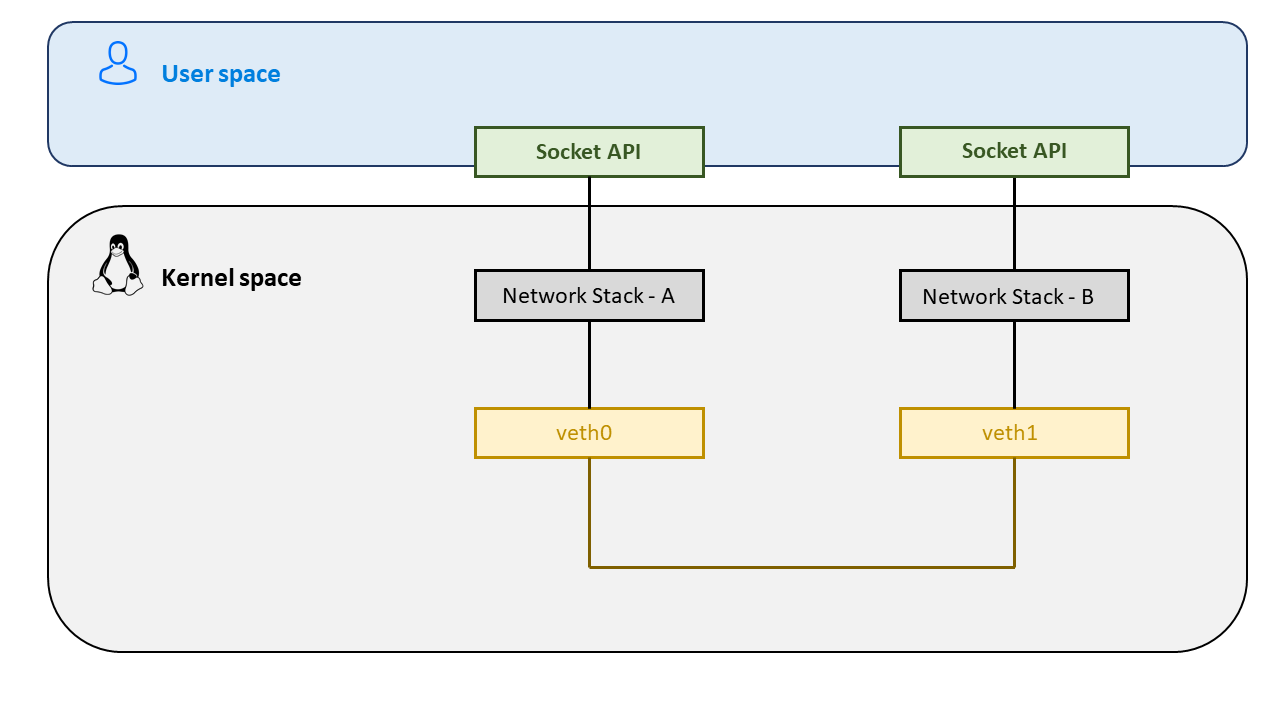
\includegraphics[width=15.5cm]{archivos/img/teoria/user_kernel.png}
    \caption{Enlace entre interfaces Veth separadas en dos Network Namespaces}
    \label{fig:linuxNet_veth}
\end{figure}

%%%%%%%%%%%%%%%%%%%%%%%%%%%%%%%%%%%%%%%%%%%%%%%%%%%%%%%%%%%%%%%%%%%%%%%%%%%%%%%%%%%%%%%%%%%%%%%%%%%%%
% Mininet & Mininet-Wifi
\section{Mininet y Mininet-WiFi}
\label{sec:mininet}

En esta sección se abordará el marco teórico relacionado con las principales herramientas de emulación utilizadas en este proyecto. Se prestará especial atención a Mininet, que es la herramienta principal y la base sobre la cual han surgido otras herramientas de emulación, como Mininet-WiFi y Mininet-IoT.\\

\subsection{Mininet}

Mininet es una herramienta utilizada para emular redes, principalmente del tipo SDN (Software-Defined Networking). Permite emular hosts, routers, switches y enlaces en una sola máquina a un coste reducido, siempre y cuando se cuente con el Kernel de Linux en dicha máquina. Para lograr esto, Mininet utiliza una forma de virtualización "ligera" que aprovecha las capacidades del Kernel de Linux para virtualizar recursos, como las \textit{Namespaces} (consultar \ref{namespaces}) \cite{lantz2010network}.\\
\\
La cantidad de recursos virtualizados dependerá de las características de cada nodo, y esto también afectará el rendimiento de la emulación. Por ejemplo, los nodos tipo \texttt{Host} en Mininet requieren el uso de una \textit{Network Namespace}, lo que les proporciona su propio \textit{stack} de red y los hace completamente independientes\footnote{En lo que respecta a Networking} del sistema y otros nodos en la red emulada. Sin embargo, por defecto, todos los nodos \texttt{Host} comparten el sistema de archivos, la numeración de procesos (PIDs), los usuarios, etc. En términos técnicos, no están completamente aislados como un host real. Esto se debe a que Mininet virtualiza solo los recursos necesarios para llevar a cabo la emulación, lo que mejora el rendimiento y permite que máquinas con recursos limitados puedan realizar la emulación \cite{lantz2010network}.\\
\\
En cuanto a la creación de topologías en Mininet, existen dos enfoques. El primero es utilizar la API escrita en Python para interactuar con las clases de Mininet. Con esta API, se puede construir la topología importando los módulos y clases necesarios para definirla en un script de Python. El segundo enfoque es utilizar la herramienta llamada \textbf{MiniEdit}, que proporciona una interfaz gráfica (GUI) donde los usuarios pueden crear la topología arrastrando y soltando nodos de red. Desde la misma GUI, se puede exportar la topología generada a un archivo (\texttt{*.mn}) para recuperarla más tarde o a un script en Python (\texttt{*.py}) para cargarla en el intérprete de Python cuando sea necesario. Esta herramienta es especialmente útil para aquellos que no tienen conocimientos de programación en Python pero desean utilizar el emulador, lo que representa una ventaja significativa \cite{lantz2010network}.\\

Por lo tanto, se puede concluir que los aspectos más fuertes de Mininet son los siguientes puntos:

\begin{itemize}
    \item Mininet es rápido gracias a su diseño basado en \textit{Namespaces}, lo que permite una gestión eficiente de los recursos. En la sección \ref{namespaces}, se explica cómo se lleva a cabo esta gestión.
    \item Mininet no consume recursos en exceso, ya que virtualiza únicamente los componentes necesarios para la emulación. Además, se pueden establecer límites máximos de recursos para la emulación en caso de ser necesario.
    \item Mininet brinda libertad al usuario para crear topologías y escenarios personalizados utilizando la API en Python de Mininet. Estos escenarios pueden ser fácilmente transferidos a otra máquina, ya que solo se requiere compartir el script que describe la topología. Es importante tener en cuenta que los resultados de las pruebas pueden variar entre diferentes máquinas, ya que Mininet emula la red en lugar de simularla. Por lo tanto, los resultados dependerán de las condiciones de la máquina donde se ejecuten las pruebas.
\end{itemize}

Aunque Mininet ofrece muchas ventajas, también tiene una limitación importante que debe tenerse en cuenta. Como se mencionó anteriormente, Mininet utiliza una forma de virtualización ``ligera" basada en las \textit{Namespaces} del Kernel de Linux. Si bien esta decisión de diseño proporciona beneficios significativos en términos de rendimiento al aprovechar el propio sistema operativo para virtualizar recursos, surge un problema cuando se intenta exportar el emulador a otra plataforma con un sistema operativo diferente. Es posible que este sistema operativo no admita un equivalente funcional a las \textit{Namespaces} de Linux o, incluso si lo hace, su API para utilizarlas puede ser completamente diferente. Esto puede dificultar o incluso impedir la ejecución de Mininet en plataformas que no porten el kernel de Linux.


\subsection{Funcionamiento de Mininet}

Anteriormente se mencionó que Mininet utiliza \textit{Network Namespaces} como método para virtualizar \textit{stacks} de red independientes y así emular redes con un costo mínimo. En la figura \ref{fig:mininet_arch}, se muestra la arquitectura interna de Mininet para una topología compuesta por dos nodos \texttt{Host} y un software switch conectado por TCP a un controlador remoto.\\
\\
Como se puede observar, cada nodo \texttt{Host} está aislado en su propia \textit{Namespace} de red, mientras que el switch se ejecuta en la \textit{Namespace} por defecto (root). La comunicación entre los nodos de esta topología se realiza mediante \gls{veth}s (consultar \ref{linuxVeths}), las cuales permiten emular los enlaces entre los diferentes nodos de la red.\\

%fig
\begin{figure}[ht]
    \centering
    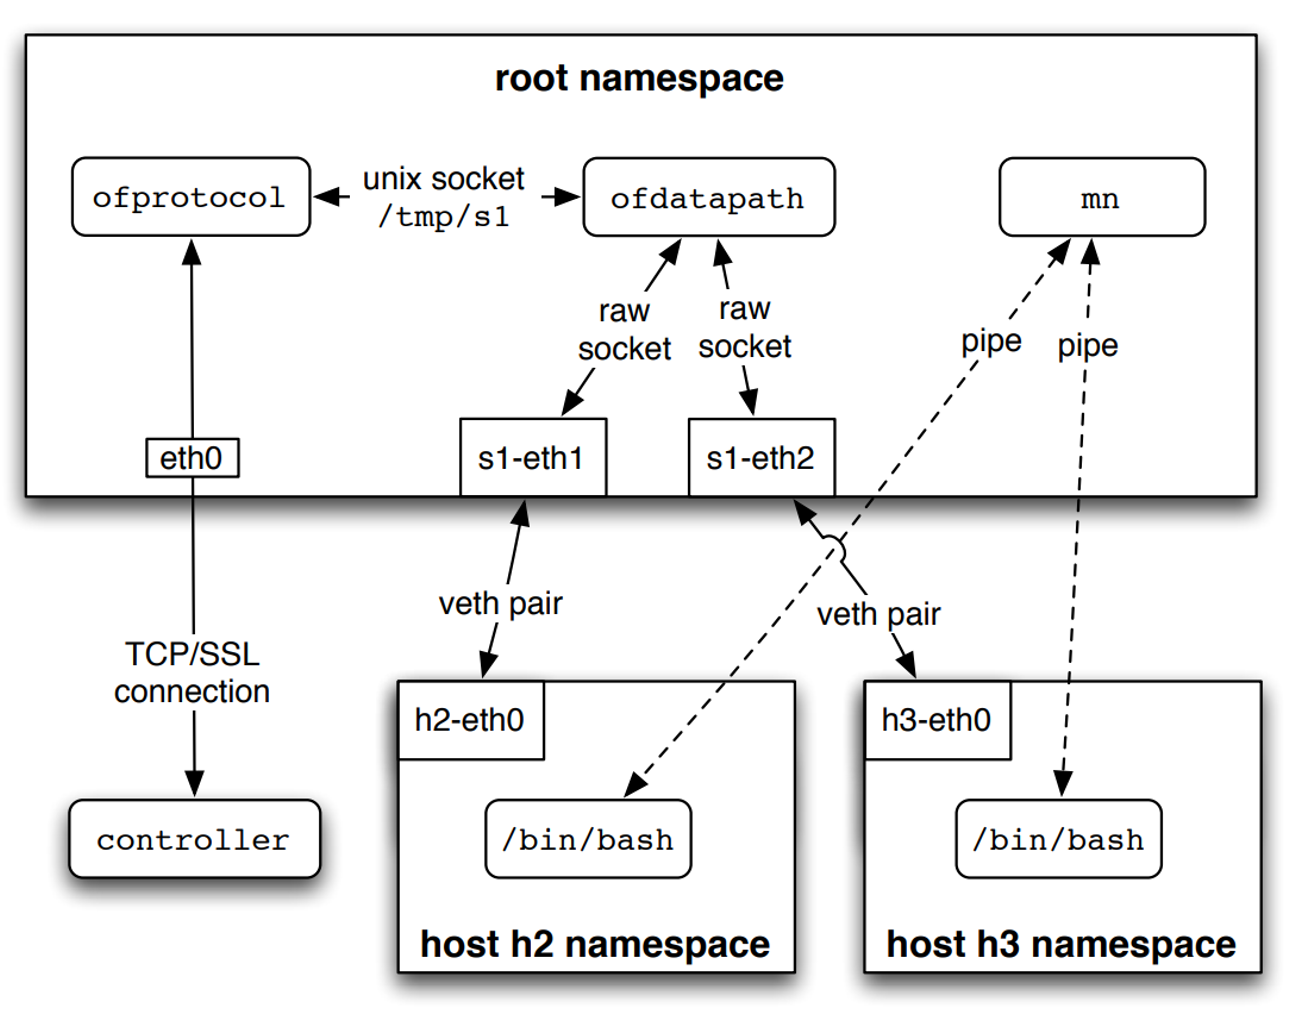
\includegraphics[width=\textwidth]{archivos/img/teoria/mn_arch.png}
    \caption{Arquitectura de Mininet \cite{heller2013reproducible}}
    \label{fig:mininet_arch}
\end{figure}

Una vez presentada toda la teoría sobre Mininet, puede surgir la pregunta de cómo se puede comprobar si realmente utiliza \textit{Network Namespaces}. Para hacerlo, lo primero que se debe hacer es crear el escenario para que Mininet pueda crear las \textit{Network Namespaces} necesarias. En este caso, se utilizará la topología mostrada en la figura \ref{fig:mininet_arch}. Para crear esta topología, solo se necesita tener Mininet instalado y seguir los pasos que se indican en el bloque \ref{code:scenarioMininet}. Una vez levantado el escenario, se debería obtener el output indicado en la figura \ref{fig:mininet_01}.


\begin{lstlisting}[language= bash, style=Consola, caption={Ejecución de Mininet con la topología por defecto},label=code:scenarioMininet]
    # Lanzamos Mininet con la topo por defecto :)
    sudo mn
    
\end{lstlisting}
\vspace{0.5cm}

\begin{figure}[ht]
    \centering
    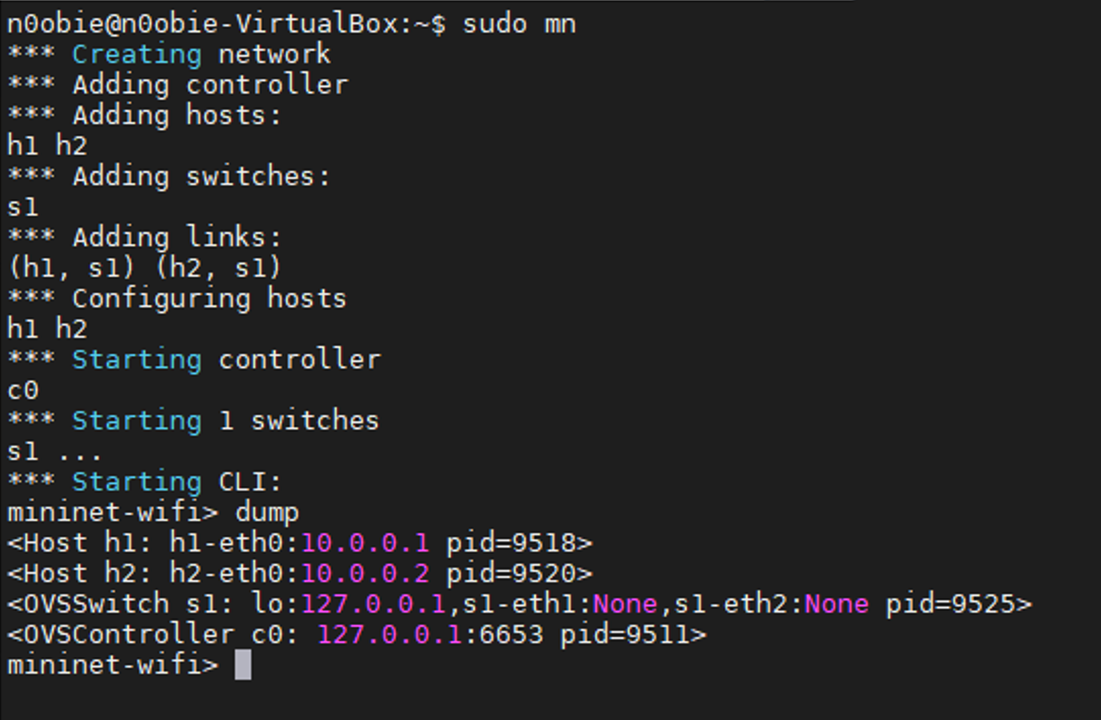
\includegraphics[width=0.7\textwidth]{archivos/img/teoria/mn_01.png}
    \caption{Salida por pantalla de la ejecución de la topología por defecto}
    \label{fig:mininet_01}
\end{figure}

Ahora que hemos creado el escenario, podemos verificar si hay \textit{Network Namespaces} en el sistema utilizando el conjunto de herramientas iproute2 (consultar \ref{iproute2}). El comando más utilizado para listar las \textit{Network Namespaces} utilizando el módulo \textbf{netns} se muestra en el bloque \ref{code:MininetNs}.


\begin{lstlisting}[language= bash, style=Consola, caption={Listar Named Network Namespaces},label=code:MininetNs]
    # Listamos las network namespaces con Nombre! ojito :)
    sudo ip netns list
\end{lstlisting}
\vspace{0.5cm}

\begin{figure}[ht]
    \centering
    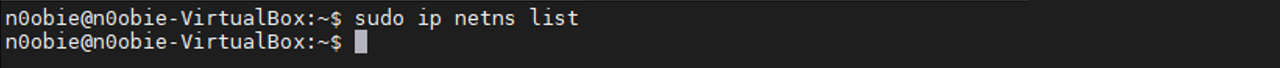
\includegraphics[width=\textwidth]{archivos/img/teoria/mn_02.png}
    \caption{Listado de Named Network Namespaces existentes en el sistema}
    \label{fig:mininet_02}
\end{figure}


Al observar la figura \ref{fig:mininet_02}, no parece haber ninguna \textit{Network Namespace} en el sistema. Entonces, ¿dónde está el problema? La razón por la que el comando \texttt{ip netns list} no muestra información es que Mininet no está creando el enlace simbólico (\textit{softlink}) necesario para que la herramienta pueda listar las \textit{Network Namespaces}. Según la documentación del comando, este lee desde la ruta \texttt{/var/run/netns/}, donde se encuentran todas las \textit{Network Namespaces} con nombre. Estas Netns son aquellas en las que se ha realizado un \textit{bindmount} con su nombre en ese directorio para que persistan incluso si no hay ningún proceso en ejecución en ellas.Como se mencionó anteriormente, las \textit{Namespaces} tienen una vida finita y solo existen mientras estén referenciadas (consulte la tabla \ref{tab:linux_ns}). Por lo tanto, si no se cumple ninguna condición de referencia, la \textit{Namespace} en cuestión se elimina.\\
\\
Mininet se encarga de recrear la red emulada y, cuando el usuario finaliza la emulación, la red emulada debe desaparecer. Este proceso debe ser lo más rápido y eficiente posible para brindar una mejor experiencia al usuario. La naturaleza del diseño de Mininet sugiere que la creación y destrucción de las \textit{Network Namespaces} están asociadas con la primera condición de referencia de una \textit{Namespace}.\\
\\
En otras palabras, no tendría sentido realizar enlaces o enlaces simbólicos que luego se deban eliminar, ya que esto implicaría una carga de trabajo significativa para emulaciones de redes grandes y aumentaría el tiempo necesario para limpiar el sistema una vez finalizada la emulación. Además, hay que tener en cuenta que existe una condición que se adapta bien a las necesidades de Mininet: solo se requiere un proceso en ejecución por cada \textit{Network Namespace}, y al realizar la limpieza, solo se deben finalizar los procesos que mantienen las \textit{Network Namespaces}. Cuando no haya más procesos en ejecución en una \textit{Namespace}, el kernel se encargará de eliminarla.\\
\\
De acuerdo con el razonamiento expuesto, se deberían ver varios procesos que se crean al iniciar el escenario en Mininet. Cada uno de estos procesos deberá tener un archivo de \textit{Network Namespace} (\texttt{/proc/{pid}/ns/net}) con un número de nodo único (\textit{inode}) para los procesos que se ejecutan en diferentes \textit{Network Namespaces}.\\

\begin{figure}[ht]
    \centering
    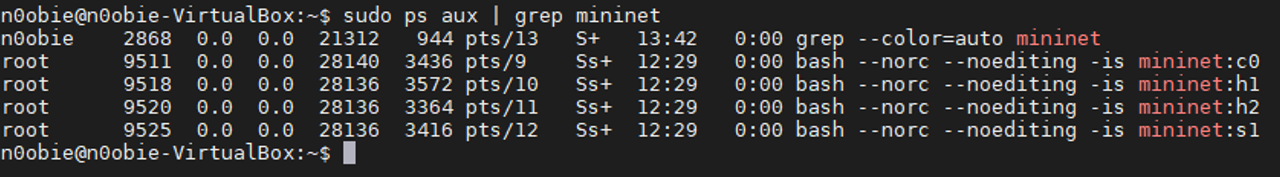
\includegraphics[width=\textwidth]{archivos/img/teoria/mn_03.png}
    \caption{Listado de procesos con referencias a Mininet}
    \label{fig:mininet_03}
\end{figure}

Si examinamos el archivo \texttt{/proc/{pid}/ns/net} para cada proceso mencionado en la figura \ref{fig:mininet_03}, podremos determinar cuáles de ellos se encuentran en una \textit{Network Namespace} distinta, según el valor del \textit{inode}. Por ejemplo, verifiquemos los procesos asociados a los \texttt{Host1} y \texttt{Host2}.\\


\begin{figure}[ht]
    \centering
    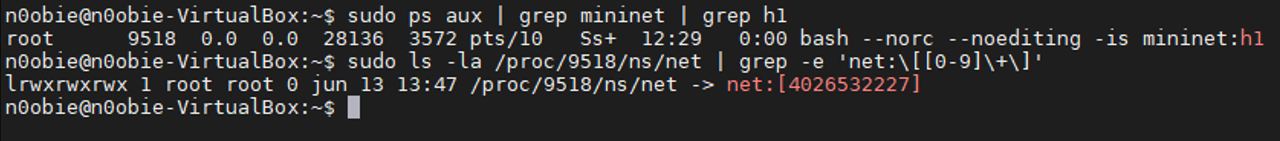
\includegraphics[width=\textwidth]{archivos/img/teoria/mn_04.png}
    \caption{Información de contexto sobre el proceso del Host1}
    \label{fig:mininet_04}
\end{figure}

\newpage

\begin{figure}[ht]
    \centering
    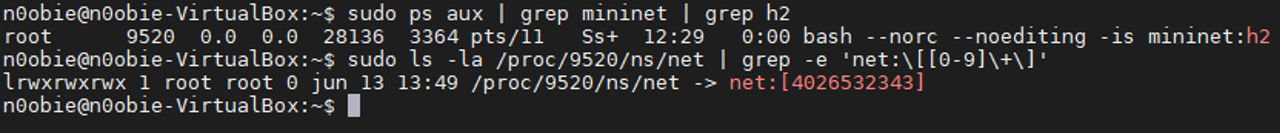
\includegraphics[width=\textwidth]{archivos/img/teoria/mn_05.png}
    \caption{Información de contexto sobre el proceso del Host2}
    \label{fig:mininet_05}
\end{figure}

Como se puede observar, hay diferentes \textit{inodes}, archivos distintos y \textit{Network namespaces} diferentes. Esta prueba demuestra cómo Mininet utiliza procesos de bash para mantener las \textit{Network Namespaces} de los nodos que lo requieren.


\subsection{Mininet-WiFi}

Mininet-WiFi \cite{7367387} es un emulador de redes inalámbricas diseñado principalmente para trabajar bajo el estándar \texttt{ieee80211}. Esta herramienta nació de Mininet, es decir, es un \textit{fork} de la misma. Por ello, comparten todas las bases sobre virtualización ``ligera" haciendo uso de \textit{Namespaces} y \gls{veth}s, por tanto, todos los scripts de Mininet son compatibles en Mininet-WiFi. \\
\par
Esto es así ya que toda la funcionalidad wireless es un añadido sobre la base que desarrollaron para Mininet. Los desarrolladores de Mininet-WiFi se valieron del subsistema wireless del Kernel de Linux y del módulo mac80211\_hwsim, para conseguir emular las interfaces y el supuesto medio inalámbrico. Para más información sobre esta herramienta se recomienda ir al \textbf{punto} \ref{mn-wifi_bmv2_integration}, donde se hace un análisis profundo sobre las jerarquías de clases añadidas en Mininet-WiFi, como opera internamente y como se comunica con el módulo en el kernel para generar los escenarios inalámbricos.



\subsection{Mininet-IoT}
\label{mininetIoT}

La herramienta Mininet-IoT \cite{mininetIOT} es un emulador de redes de baja capacidad diseñado para trabajar en conjunto bajo el estándar \texttt{ieee802154} y la capa de adaptación 6LoWPAN. Esta herramienta nació de Mininet-WiFi, que a su vez nació de Mininet, por lo que en la práctica, Mininet-IoT comparte todas las técnicas de virtualización ``ligera" de Mininet. Al heredar de Mininet-WiFi y Mininet, todos los scripts para desplegar topologías alámbricas y WiFi son compatibles en Mininet-IoT.  \\
\par

La gran diferencia entre Mininet-IoT y Mininet-WiFi, radica en el módulo que emplean para conseguir emular las interfaces y el supuesto medio inalámbrico. Mininet-WiFi hace uso del módulo mac80211\_hwsim, mientras que Mininet-IoT hace uso del módulo del Kernel mac802154\_hwsim (es necesario tener una versión del Kernel superior a la \texttt{4.18.x} para obtener dicho modulo). Toda la gestión de nodos, interfaces y enlaces es exactamente la misma a la de Mininet-WiFi. Por ello, Ramon Fontes (principal desarrollador de la herramienta), creó una clase agnóstica para gestionar módulos del Kernel en Mininet-WiFi, y migró todo el proyecto de Mininet-IoT a Mininet-WiFi. De esta forma, el mantenimiento del \textit{core} que compartían ambas herramientas se hacía únicamente en un proyecto, y daba la posibilidad al usuario de Mininet-WiFi de establecer enlaces de baja capacidad en sus topologías inalámbricas.

%%%%%%%%%%%%%%%%%%%%%%%%%%%%%%%%%%%%%%%%%%%%%%%%%%%%%%%%%%%%%%%%%%%%%%%%%%%%%%%%%%%%%%%%%%%%%%%%%%%%%
% Contiki-ng
\section{Contiki-ng}
\label{sec:contikiNG}

Contiki es un sistema operativo diseñado específicamente para dispositivos de baja capacidad, como sensores. Fue desarrollado por Adam Dunkels en colaboración con Bjorn Gronvall y Thiemo Voigt en 2002. A lo largo de los años, el proyecto Contiki ha crecido enormemente y ha involucrado a numerosas empresas y cientos de colaboradores en su repositorio de GitHub\footnote{\url{https://github.com/contiki-os/contiki}}. El objetivo principal de Contiki era proporcionar a los nodos de las redes de sensores inalámbricos (WSN) un sistema operativo liviano capaz de cargar y descargar servicios de forma dinámica \cite{1367266}.\\
\\
El kernel de Contiki se basa en un modelo orientado a eventos y admite multitarea con prelación. Está escrito en lenguaje C y ha sido portado a diversas arquitecturas de microcontroladores, como el MSP430 de Texas Instruments y sus variantes.\\
\\
En un sistema que ejecuta Contiki, este se divide en dos partes claramente diferenciadas, como se muestra en la Figura \ref{fig:contikiParts}: el núcleo (\textit{core}) y los programas o servicios cargados. Esta partición se realiza durante la etapa de compilación y es independiente del objetivo (target) donde se desplegará el sistema. El núcleo (\textit{core}) incluye el propio kernel, un conjunto de servicios base (como temporizadores y controladores), bibliotecas, controladores y el stack de comunicación. Los programas o servicios cargados se mapean en memoria mediante el cargador del kernel durante el tiempo de ejecución.\\


% Foto 
\begin{figure}[ht]
    \centering
    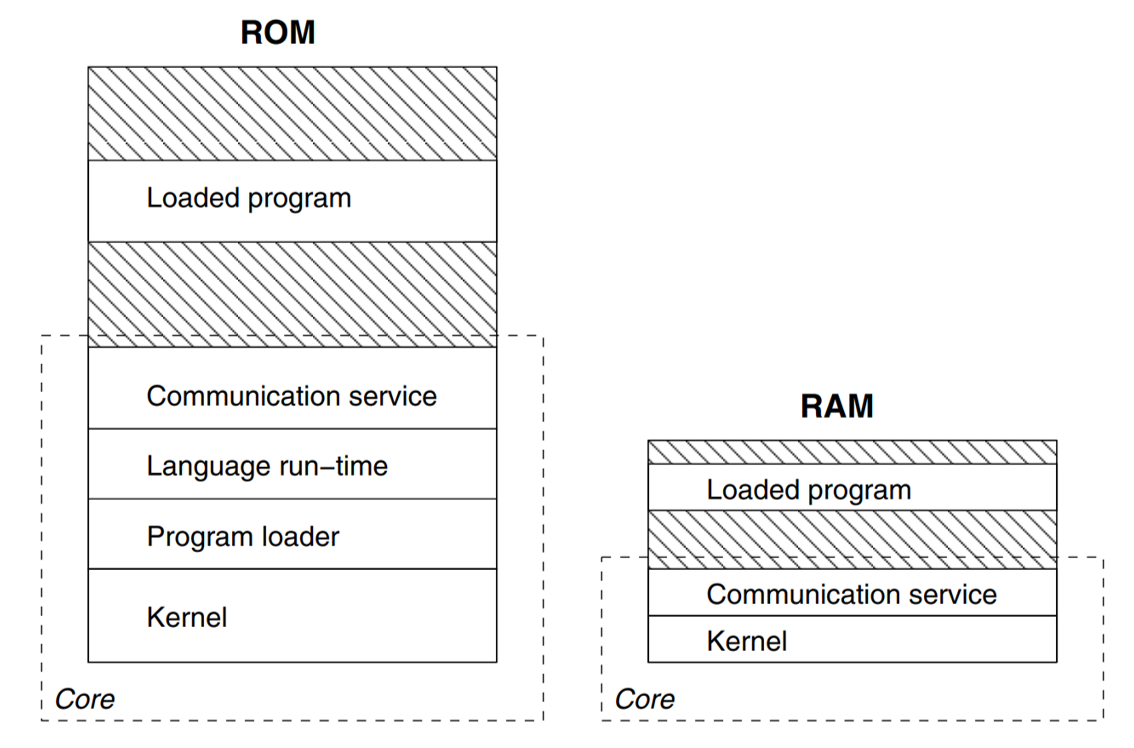
\includegraphics[width=0.8\textwidth]{archivos/img/teoria/contiki.png}
    \caption{Gestión de la memoria en un sistema con Contiki OS \cite{1367266}}
    \label{fig:contikiParts}
\end{figure}


En los últimos años ha surgido un nuevo proyecto llamado \textbf{Contiki-ng}\footnote{\url{https://github.com/contiki-ng/contiki-ng}}, el cual es un fork del sistema operativo Contiki. Este proyecto ha ganado popularidad y ha superado a su predecesor con el eslogan ``Contiki-NG: El sistema operativo para dispositivos IoT de próxima generación". Actualmente, toda la comunidad de Contiki se está centrando en este nuevo proyecto, el cual proporciona un stack de comunicación más compatible con las especificaciones RFC, ofrece soporte para protocolos como IPv6/6LoWPAN y 6TiSCH, y se está volviendo cada vez más popular por su capacidad de brindar soporte a microcontroladores con arquitectura ARM \cite{kurniawan2018practical}.

\subsection{Simulador Cooja}

El flujo de trabajo con Contiki o Contiki-ng varía dependiendo de si se trabaja con hardware real o si se realiza una simulación de los programas desarrollados. En el caso de trabajar con hardware real, el proceso consiste en compilar el sistema operativo y los programas específicos utilizando el objetivo (target) correspondiente, lo que generará un archivo binario que se puede cargar en la memoria del hardware.\\
\\
Por otro lado, si se opta por la simulación, se utilizará el simulador llamado Cooja\footnote{\url{https://github.com/contiki-ng/cooja/tree/master}}. Cooja es un simulador escrito en Java que permite \textbf{simular} una serie de nodos \gls{iot}. Al simular, es posible observar el comportamiento del programa desarrollado en diferentes plataformas. El proceso de compilación del núcleo (core) de Contiki y los programas desarrollados está integrado en el propio simulador, lo que facilita al usuario la compilación de sus programas para diferentes tipos de nodos. Cada simulación se puede guardar en un archivo con extensión \texttt{*.csc}, que almacena todos los datos de la simulación, como la semilla (\textit{seed}), las posiciones y los tipos de nodos, utilizando una estructura XML.\\
\\
De esta manera, tanto si se trabaja con hardware real como si se realiza una simulación, Contiki y Contiki-ng ofrecen herramientas y entornos integrados que permiten desarrollar y probar programas para sistemas embebidos y dispositivos \gls{iot}. A continuación, en la figura \ref{fig:cooja}, se indica la interfaz gráfica del simulador.

\begin{figure}[ht]
    \centering
    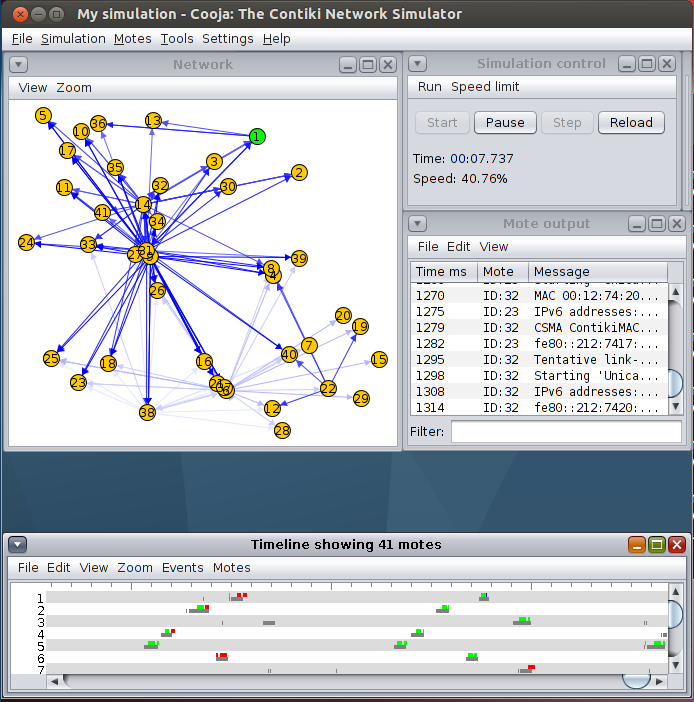
\includegraphics[width=0.6\textwidth]{archivos/img/teoria/cooja.png}
    \caption{Interfaz gráfica del simulador Cooja \cite{cooja1}}
    \label{fig:cooja}
\end{figure}



%%%%%%%%%%%%%%%%%%%%%%%%%%%%%%%%%%%%%%%%%%%%%%%%%%%%%%%%%%%%%%%%%%%%%%%%%%%%%%%%%%%%%%%%%%%%%%%%%%%%%
% Contribuciones en repos - Github
\section{Contribuciones en GitHub}
\label{sec:estadoArte_github}


El proyecto GitHub es una plataforma que proporciona alojamiento de repositorios. En el presente Trabajo de Fin de Máster (TFM), se utilizará la herramienta de control de versiones Git\footnote{\url{https://git-scm.com/}}, junto con GitHub como plataforma para alojar el código desarrollado. Sin embargo, GitHub no se utilizará únicamente para almacenar el código del TFM, sino que se aprovechará su carácter público para ofrecer documentación y ejemplos a todos los usuarios interesados que visiten el repositorio. \\
\par
\begin{itemize}
    \item Enlace al repositorio del \gls{tfm}: \url{https://github.com/davidcawork/TFM}
    \item Enlace al repositorio de la tesis: \url{https://github.com/davidcawork/tfm-thesis}
\end{itemize}
\vspace{0.5cm}

El repositorio incluye ficheros \texttt{README.md} en todos los directorios, que proporcionan explicaciones y análisis teóricos que permiten al visitante comprender la naturaleza de las pruebas, sus objetivos y las conclusiones que se pueden extraer de ellas. El propósito del repositorio es doble, ya que no solo almacena el código, sino que también ayuda a difundir los contenidos del proyecto. Además, se han ofrecido contribuciones útiles que pueden beneficiar a otros repositorios a través de solicitudes de extracción (pull requests). Durante este proyecto se ha contribuido de forma muy activa en varios proyectos opensource dado que la naturaleza del mismo abarcaba varias herramientas.  La tabla \ref{tab:githubContr} muestra todas las contribuciones realizadas.\\
\\

\begin{table}[ht]
    \centering
    \resizebox{\textwidth}{!}{%
        \begin{tabular}{|l|l|}
            \hline
            \rowcolor[HTML]{EFEFEF}
            \multicolumn{1}{|c|}{\cellcolor[HTML]{EFEFEF}{\color[HTML]{24292E} \textbf{Contribución}}} & \multicolumn{1}{c|}{\cellcolor[HTML]{EFEFEF}{\color[HTML]{24292E} \textbf{Enlace al Pull-Request}}} \\ \hline
            Dar soporte al bmv2 entorno P4 en Mininet-WiFi                                             & \url{https://github.com/intrig-unicamp/mininet-wifi/pull/302}                                       \\ \hline
            Arreglar la compilación del BOFUSS en Mininet-WiFi                                         & \url{https://github.com/intrig-unicamp/mininet-wifi/pull/495}                                       \\ \hline
            Aclarar el uso de ONOS-gui                                                                 & \url{https://groups.google.com/a/opennetworking.org/g/onos-dev/c/mbfyCaoeCdU}                       \\ \hline
            Resolver problema interfaz dpctl con el BOFUSS                                             & \url{https://github.com/mininet/mininet/issues/745}                                                 \\ \hline
            Dar escenarios funcionales en la 22.04 de Mininet con Onos                                 & \url{https://groups.google.com/a/opennetworking.org/g/onos-dev/c/a0VjA0Xw_-M}                       \\ \hline
        \end{tabular}%
    }
    \caption{Resumen de contribuciones realizadas durante todo el proyecto del \gls{tfm}}
    \label{tab:githubContr}
\end{table}
